\graphicspath{{figtema2/}}

\chapter{Organizaci\'on y descripci\'on de datos estad\'\i sticos}

El primer paso en la realizaci\'on de un estudio estad\'\i stico
consiste en la recopilaci\'on de los datos que caracterizan el tema
bajo estudio. Estos datos se obtienen de m\'ultiples observaciones
de los elementos de una poblaci\'on o una muestra. 

En ocasiones, la recopilaci\'on de datos est� controlada por el equipo 
de personas responsable del estudio. Por ejemplo, en un estudio sobre
la satisfacci\'on de los consumidores de un determinado producto
de limpieza se pueden hacer encuestas a un cierto n\'umero de 
clientes de grandes centros comerciales, o solicitar a los compradores
del producto el env\'\i o de un cuestionario de satisfacci\'on.

En algunas ocasiones, no obstante el estudio puede hacerse a partir
de datos recopilados por organismos o instituciones independientes.
Tal ser\'\i a el caso de un estudio sobre siniestralidad laboral,
donde los datos podr\'\i an proceder del Ministerio de Trabajo.

Una fuente importante de datos estad\'\i sticos a nivel nacional la 
ofrece el Instituto Nacional de Estad\'\i stica. A trav\'es de su p\'agina 
web (\url{www.ine.es}) se pueden obtener datos oficiales sobre econom\'\i a,
sociedad, medio ambiente, etc. En la secci\'on \ref{secINE} del tema
explicamos como acceder a estos datos. Tambi\'en la Direcci\'on General
de Tr\'afico en su p\'agina web (\url{www.dgt.es}) ofrece datos estad\'isticos
sobre seguridad vial. En Baleares, una fuente importante de datos 
oficiales es el Institut d'Estad\'istica de les Illes Balears (IBESTAT,
\url{http://www.caib.es/ibae/ibae.htm}).

\vskip 0.3 cm
Existen protocolos de recogida de datos que aseguran que los datos recopilados
a partir de una muestra representan de manera fiel a toda la poblaci\'on bajo estudio. 
En este curso no estudiaremos tales protocolos sino que consideraremos que 
ya disponemos de una serie de datos y veremos c\'omo organizarlos e interpretarlos.

En el presente tema explicaremos diferentes maneras de organizar y re\-pre\-sen\-tar
los datos obtenidos de una manera visualmente agradable y que facilite su posterior
interpretaci\'on. Exiten dos formas b\'asicas de organizar los datos: mediante tablas
y mediante gr�ficas. En estas tablas y gr\'aficas se muestran una serie de par\'ametros 
calculados a partir de los datos originales (denominados tambi\'en \textbf{datos brutos}
o \textbf{datos en bruto}, \textit{raw data} en ingl�s).
A continuaci\'on definimos los par\'ametros m\'as habituales
y explicamos c\'omo representarlos mediante tablas y gr\'aficas.

\section{Frecuencias y porcentajes}
%El primer par\'ametro que definiremos es la \textbf{frecuencia absoluta}. 
%Consideremos el siguiente ejemplo: deseamos hacer un estudio sobre la inmigraci\'on
%y tomamos una muestra formada por 1000 inmigrantes a los que preguntamos por su nacionalidad.
%Supongamos que los resultados obtenidos son: 350 personas de Colombia, 250 de Ecuador, 120
%de Per\'u, 100 de Argentina, 80 de Ruman\'ia, 70 de Marruecos y 30 de Senegal. 
%Las cantidades 350, 250, 120, 100, 80, 70 y 30, que representan la cantidad de personas
%de cada nacionalidad se denominan \textbf{frecuencias absolutas}.

El primer par\'ametro que definiremos es la \textbf{frecuencia absoluta}. 
Con\-si\-de\-re\-mos el siguiente ejemplo: deseamos hacer un estudio sobre la inmigraci\'on
y tomamos una muestra formada por 1000 inmigrantes a los que preguntamos por su nacionalidad.
Supongamos que algunos de los resultados obtenidos son los que se muestran en la tabla \ref{tabla0}. 
\vskip 0.2 cm
\begin{table}
\caption{Inmigrantes seg\'un su nacionalidad. Datos brutos.}
\label{tabla0}
\begin{center}
\begin{tabular}{c|c}
Persona & Nacionalidad \\ \hline
1 & Colombia \\
2 & Ruman\'ia \\
3 & Colombia \\
4 & Senegal \\
5 & Per\'u \\
6 & Colombia \\
7 & Ecuador \\
8 & Ecuador \\
9 & Marruecos \\
10 & Per\'u \\
$\vdots$ & $\vdots$ \\
998 & Colombia \\
999 & Per\'u \\
1000 & Ruman\'ia
\end{tabular}
\end{center}
\end{table}

La tabla \ref{tabla0} consta de 1000 datos, de los cuales se muestran los 10 primeros
y los 3 \'ultimos. Leer los datos de una tabla tan grande es complicado. Una manera
de mostrar los datos de una forma m\'as resumida consiste en contar cu\'antas
personas hay de cada nacionalidad. Supongamos por ejemplo que tuvi\'eramos:
350 personas de Colombia, 250 de Ecuador, 120
de Per\'u, 100 de Argentina, 80 de Ruman\'ia, 70 de Marruecos y 30 de Senegal. 
Las cantidades 350, 250, 120, 100, 80, 70 y 30, que re\-pre\-sen\-tan la cantidad de personas
de cada nacionalidad, se denominan \textbf{frecuencias absolutas}.
Las frecuencias absolutas resumen los datos 
brutos. En este ejemplo, los 7 valores de las frecuencias absolutas describen el 
comportamiento de 1000 valores de datos brutos.


En general, dada una variable de un estudio estad\'\i stico (en nuestro ejemplo la variable
es \textit{Nacionalidad}), la frecuencia absoluta de los valores de la variable es el
n\'umero de veces que aparece cada valor en la muestra con\-si\-de\-ra\-da.

\vskip 0.3 cm
Otro ejemplo es el siguiente: se desea estudiar la edad de los es\-tu\-dian\-tes de la
UIB (variable: \textit{Edad}) y se encuentran los siguientes valores (ya agrupados en frecuencias
absolutas) para una muestra
de 626 estudiantes: 120 personas de 18 a\~nos, 150 de 19 a\~nos, 90 de 20 a\~nos, 70 de
21 a\~nos, 65 de 22 a\~nos, 50 de 23 a\~nos, 30 de 24 a\~nos, 20 de 25 a\~nos, 10 de 26 a\~nos,
7 de 27 a\~nos, 8 de 28 a\~nos, 2 de 29 a\~nos, 1 de 30 a\~nos, 1 de 34 a\~nos, 1 de 35 a\~nos y
1 de 40 a\~nos. Los valores que toma la variable \textit{Edad} en este caso son: 18, 19, 20, 21,
22, 23, 24, 25, 26, 27, 28, 29, 30, 34, 35 y 40. Y sus frecuencias absolutas respectivas son:
120, 150, 90, 70, 65, 50, 30, 20, 10, 7, 8, 2, 1, 1, 1, 1.

En general se denota como $n_i$ la frecuencia absoluta del valor $i$-\'esimo de una variable.
Por ejemplo, en el estudio sobre la inmigraci\'on, tenemos que $n_{\text{Argentina}}=100$;
y en el estudio sobre los estudiantes de la UIB $n_{25}=20$.
Observemos que la suma de todas las frecuencias absolutas es igual al tama\~no total de la muestra
(que denotamos como $N$): $\sum_i n_i=N$.

En ocasiones es habitual agrupar distintos valores de una variable en un mismo \textbf{intervalo}.
Por ejemplo, en el estudio sobre la edad en la UIB, podr\'iamos agrupar los resultados
por grupos de edad: de 18 a 21 a\~nos hay 430 estudiantes, de 22 a 25 a\~nos 165 y mayores de 25
31 estudiantes. En este caso dir\'iamos que 430, 165 y 31 son las frecuencias absolutas de los
intervalos $18-21$, $22-25$ y \textit{mayor de $25$}.
Los valores de frecuencia variar\'an con una elecci\'on distinta de los intervalos.
En la siguiente secci\'on se muestran otras dos maneras de agrupar los valores para este mismo
ejemplo.



A partir de la frecuencia absoluta se pueden definir otros par\'ametros que caracterizan la muestra:
%estad\'isticos (en ocasiones llamados simplemente \textit{estad\'isticos}):

\begin{itemize}
\item \textbf{Frecuencia relativa} o \textbf{proporci\'on}. 
\[
f_i=\frac{n_i}{N}
\]

En el ejemplo sobre la inmigraci\'on: $f_{\text{Colombia}}=\frac{350}{1000}=0,35$, 
$f_{\text{Ecuador}}=\frac{250}{1000}=0,25$, etc.

En el ejemplo sobre la edad en la UIB: $f_{18-21}=\frac{430}{626}=0,6869$, 
$f_{22-25}=\frac{165}{626}=0,2636$ y $f_{\text{mayor 25}}=\frac{25}{626}=0,0399$.

Observemos que la suma de todos los valores $f_i$ es siempre igual a 1.  

\item \textbf{Porcentaje}. Es la frecuencia relativa multiplicada por $100$.
\[
p_i=\frac{n_i}{N} \times 100 \quad \%
\]

En el ejemplo sobre la inmigraci\'on: $p_{\text{Colombia}}=35 \%$, 
$p_{\text{Ecuador}}=25 \%$, etc.

En el ejemplo sobre la edad en la UIB: $p_{18-21}=68,69 \%$, 
$p_{22-25}=26,36\%$ y $p_{\text{mayor 25}}=3,99\%$.

Observemos que la suma de todos los valores $p_i$ es siempre igual a $100$.  


\item \textbf{Frecuencia absoluta acumulada}. 
En el caso de variables ordinales o cuantitativas es posible ordenar
los valores siguiendo alg\'un criterio. En este caso, si $n_1$
representa la frecuencia absoluta del primer valor, $n_2$ la del 
segundo, etc, la frecuencia absoluta acumulada para el valor $i$
se define como
\[
N_i=\sum_{j \leq i} n_j
\]

No tiene sentido aplicar esta definici\'on al caso del ejemplo 
sobre la inmigraci\'on, pues la variable \textit{Nacionalidad}
es una variable cualitativa.

En el ejemplo sobre la edad en la UIB, si el orden de los intervalos
es $18-21$, $22-25$ y \textit{mayor $25$}:
$N_{18-21}=430$, $N_{22-25}=430+165=595$ y $N_{\text{mayor 25}}=430+165+31=626$.

Observemos que la frecuencia absoluta acumulada del \'ultimo valor de
la variable es siempre igual al tama\~no de la muestra $N$.

\item \textbf{Frecuencia relativa (proporci\'on) acumulada}. De manera similar 
al estad\'istico anterior definimos la frecuencia relativa acumulada como:
\[
F_i=\frac{N_i}{N}
\]


En el ejemplo sobre la edad en la UIB, considerando el mismo orden que en el estad\'istico
anterior: $F_{18-21}=\frac{430}{626}=0,6869$, $F_{22-25}=\frac{595}{626}=0,9505$ y 
$F_{\text{mayor 25}}=\frac{626}{626}=1$.

Se puede comprobar f\'acilmente que la frecuencia relativa acumulada para un valor $i$
es igual a la suma de las frecuencias relativas de todos los valores anteriores (incluido $i$):
$F_i=\sum_{j \leq i} f_j$.

Adem\'as, la frecuencia relativa acumulada del \'ultimo valor de
la variable es siempre igual 1.

\item \textbf{Porcentajes acumulado}. Es la frecuencia relativa acumulada multiplicada por $100$.
\[
P_i=\frac{N_i}{N} \times 100 \quad \%
\]


En el ejemplo sobre la edad en la UIB, considerando el mismo orden que en el estad\'istico
anterior: $P_{18-21}=68,69 \%$, $P_{22-25}=95,05 \%$ y $P_{\text{mayor 25}}=100 \%$.

El porcentaje acumulado del \'ultimo valor de la variable es siempre igual a $100 \%$.

\end{itemize}


\section{Tablas de frecuencia}
Los par\'ametros anteriores se pueden representar mediante tablas.
En la primera columna de la tabla se enumeran los distintos valores de la va\-ria\-ble
considerada y en las columnas siguientes se muestran las frecuencias o porcentajes
asociados a cada valor de la variable.

Para los ejemplos utilizados en la secci\'on anterior obtendr\'iamos las tablas
de frecuencias y porcentajes \ref{tabla1} y \ref{tabla2}, respectivamente.

\begin{table}[htbp]
\begin{center}
\caption{Inmigraci\'on por nacionalidades}
\label{tabla1}

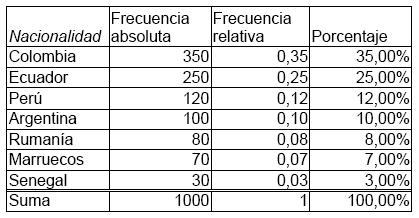
\includegraphics[width=8cm]{ejemplo1.png} 
\end{center}
\end{table}

\begin{table}[htbp]
\begin{center}
\caption{Estudiantes UIB por edad}
\label{tabla2}

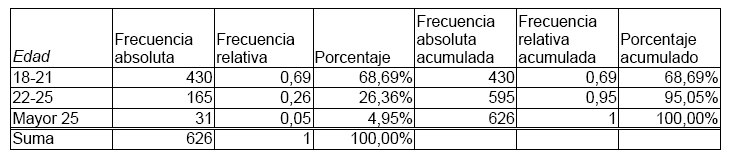
\includegraphics[width=14cm]{ejemplo2.png} 
\end{center}
\end{table}

Ya se ha comentado en la secci\'on anterior que para el ejemplo sobre la edad de los estudiantes
de la UIB podr\'ian haberse utilizado otras maneras de agrupar los valores de edad 
en intervalos.
La tablas \ref{tabla2b} y \ref{tabla2c}
muestran las frecuencias y porcentajes que obtendr\'iamos con dos agrupaciones
diferentes. En el primer caso se muestran los par\'ametros obtenidos para cada valor de 
la variable \textit{Edad} sin agrupar en intervalos.
En el segundo caso se agrupan las edades en intervalos de 2 a\~nos, salvo los \'ultimos valores 
que se agrupan como \textit{mayores de $29$ a\~nos}. 

\begin{table}[htbp]
\begin{center}
\caption{Estudiantes UIB por edad}
\label{tabla2b}

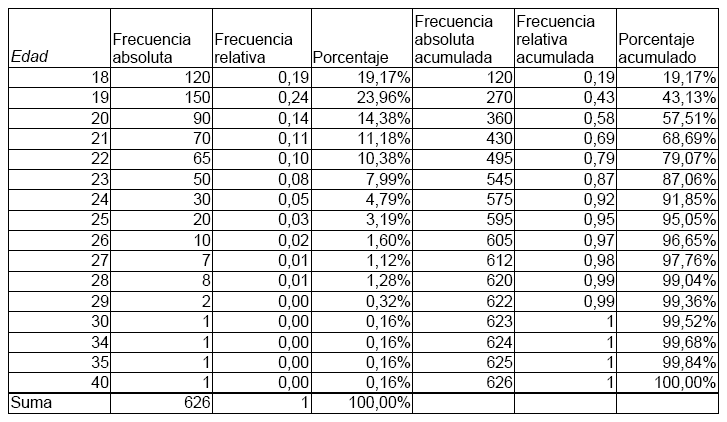
\includegraphics[width=14cm]{ejemplo2b.png} 
\end{center}
\end{table}

\begin{table}[htbp]
\begin{center}
\caption{Estudiantes UIB por edad}
\label{tabla2c}

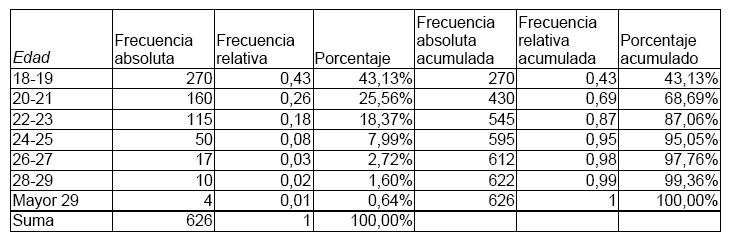
\includegraphics[width=14cm]{ejemplo2c.png} 
\end{center}
\end{table}


Observamos como los valores de la tabla \ref{tabla2b} son m\'as dif\'iciles de leer que los de 
las tablas \ref{tabla2} y \ref{tabla2c}, pues hay muchos m\'as datos. 
En cambio en las tablas \ref{tabla2} y \ref{tabla2c} se pierde el detalle de que hay m\'as
estudiantes de 19 a\~nos que de 18. En general debe buscarse un tama\~no de los intervales
que permita un compromiso entre la claridad de la representaci\'on y los detalles que ofrece. 


\section{Representaciones gr\'aficas}

La frecuencias y porcentajes de las variables estad\'isticas pueden representarse
gr\'aficamente de diversas maneras:
\begin{itemize}
\item \textbf{Diagramas de barras}. 
En este tipo de gr\'afica los valores de la variable se representan
sobre el eje horizontal y a cada valor se le asocia una barra vertical
cuya altura es proporcional a la frecuencia (absoluta o relativa) o porcentaje 
del valor. 
Las dos siguientes figuras muestran los diagramas de barras correspondientes
a los ejemplos mostrados en la secci\'on anterior.


\begin{figure}[htbp]
\begin{center}
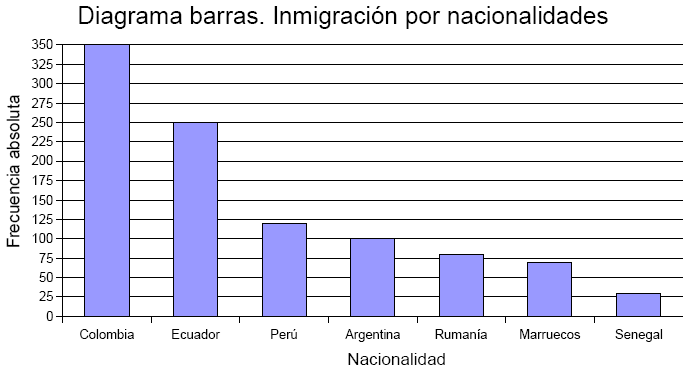
\includegraphics[width=12cm]{ejemplo1bar.png} 
\end{center}
\caption{Diagrama de barras de frecuencias absolutas de la tabla \ref{tabla1}}
\label{tabla1bar}
\end{figure}

\begin{figure}[htbp]
\begin{center}
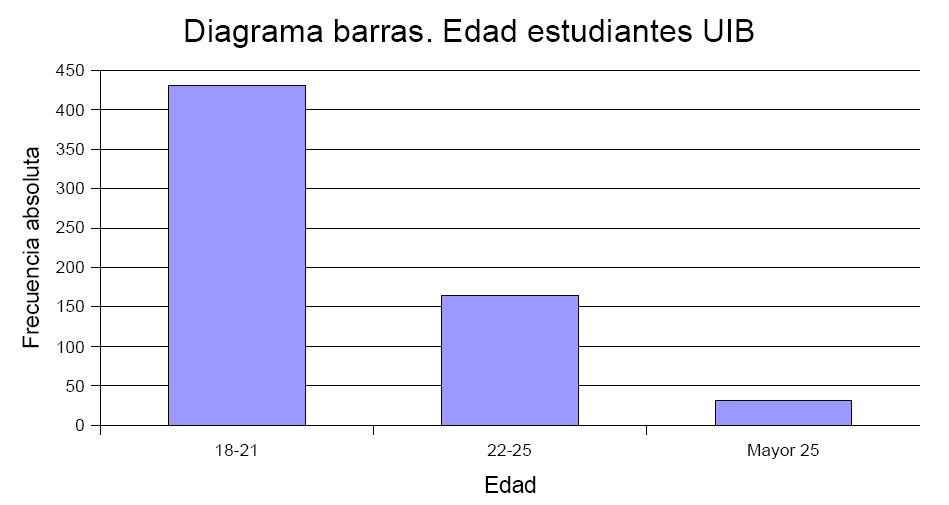
\includegraphics[width=10cm]{ejemplo2bar.png} 
\end{center}
\caption{Diagrama de barras de frecuencias absolutas de la tabla \ref{tabla2}}
\label{tabla2bar}
\end{figure}


Para el ejemplo sobre los estudiantes de la UIB se muestran tambi\'en 
(figuras \ref{tabla2bbar} y \ref{tabla2cbar}) los
diagramas correspondientes a las agrupaciones de valores de las
tablas \ref{tabla2b} y \ref{tabla2c}. Como ya se ha comentado en la secci\'on
anterior, el uso de intervalos grandes permite observar mejor la 
distribuci\'on de los valores pero impide apreciar los detalles.


\begin{figure}[htbp]
\begin{center}
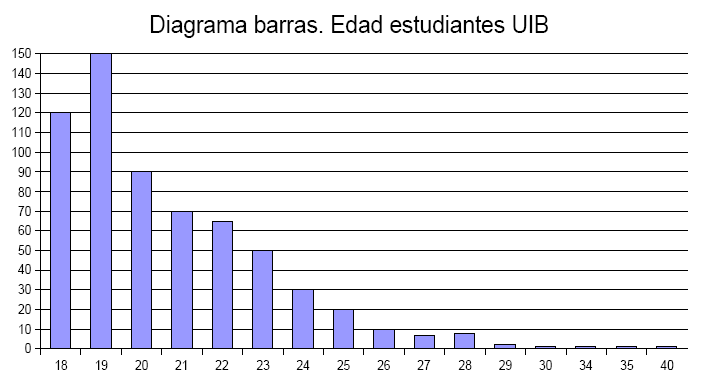
\includegraphics[width=12cm]{ejemplo2bbar.png} 
\end{center}
\caption{Diagrama de barras de frecuencias absolutas de la tabla \ref{tabla2b}}
\label{tabla2bbar}
\end{figure}

\begin{figure}[htbp]
\begin{center}
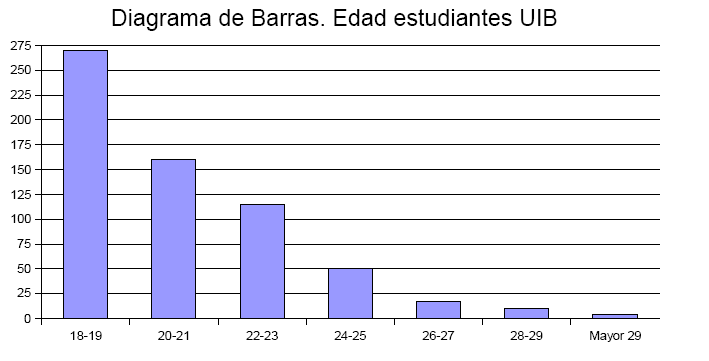
\includegraphics[width=12cm]{ejemplo2cbar.png} 
\end{center}
\caption{Diagrama de barras de frecuencias absolutas de la tabla \ref{tabla2c}}
\label{tabla2cbar}
\end{figure}




Una variante del diagrama de barras es el \textbf{diagrama de Pareto}. En este caso
las frecuencias o porcentajes est\'an ordenadas de mayor a menor y 
adem\'as se dibuja una l\'inea indicativa de la frecuencia o porcentaje acumulados.
El diagrama de Pareto correspondiente a los porcentajes del 
ejemplo sobre la edad de los estudiantes de la UIB se muestra en la figura \ref{tabla1pareto}.


\begin{figure}[htbp]
\begin{center}
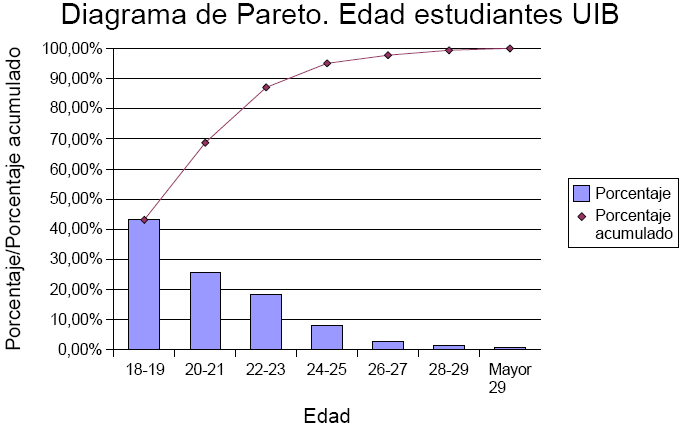
\includegraphics[width=12cm]{ejemplo2cpareto.png} 
\end{center}
\caption{Diagrama de Pareto de porcentajes y porcentajes acumulados de la tabla \ref{tabla2c}}
\label{tabla1pareto}
\end{figure}

\item \textbf{Diagramas de barras dobles}
Las tablas mostradas en la secci\'on anterior mostraban valores de frecuencia relativos a
una \'unica variable. En ocasiones se desea mostrar de manera conjunta los datos de dos
variables, para ello se emplean los diagramas de barras dobles. 
En el ejemplo 2 de la secci�n \ref{sectabgraford} (figura \ref{calcbarrasej2}) se
muestra un ejemplo de este tipo de diagramas.

\item \textbf{Histogramas}. Un histograma es un gr\'afico que describe
las frecuencias absolutas de una variable cuantitativa mediante barras 
contiguas de \'area proporcional a la frecuencia representada.
Para el ejemplo de la edad de los estudiantes de la UIB (tabla \ref{tabla2}) el histograma
correspondiente se muestra en la figura \ref{tabla2his}.


\begin{figure}[htbp]
\begin{center}
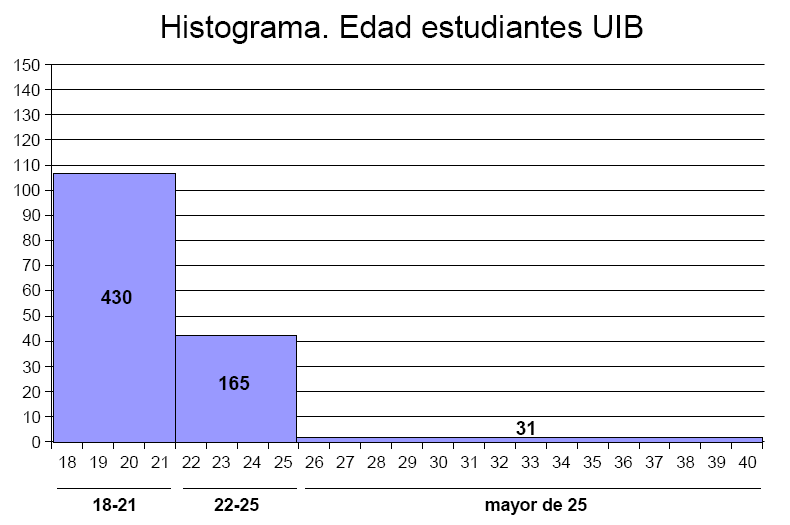
\includegraphics[width=12cm]{ejemplo2his.png} 
\end{center}
\caption{Histograma de frecuencias absolutas de la tabla \ref{tabla1}}
\label{tabla2his}
\end{figure}

El eje horizontal del histograma representa los distintos intervalos de valores
considerados. En el ejemplo las edades est\'an agrupadas en periodos de 
4 a\~nos (salvo el \'ultimo intervalo ``mayores de 25''), 
los dos siguientes histogramas (figuras \ref{tabla2bhis} y \ref{tabla2chis})
muestran el resultado agrupando en periodos de 1 y 2 a\~nos, 
respectivamente (tablas \ref{tabla2b} y \ref{tabla2c}).


\begin{figure}[htbp]
\begin{center}
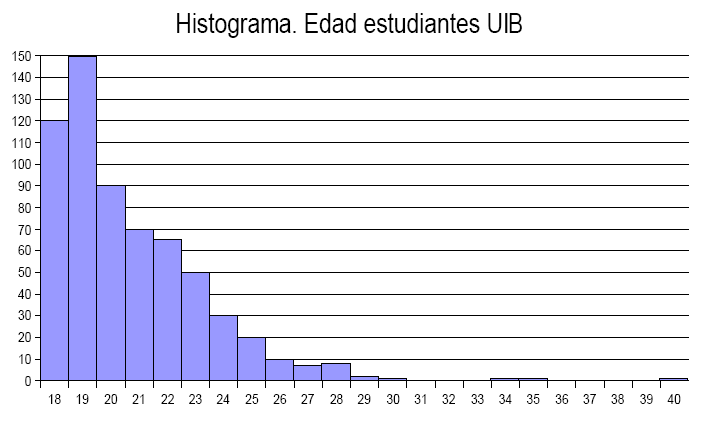
\includegraphics[width=12cm]{ejemplo2bhis.png} 
\end{center}
\caption{Histograma de frecuencias absolutas de la tabla \ref{tabla2b}}
\label{tabla2bhis}
\end{figure}

\begin{figure}[htbp]
\begin{center}
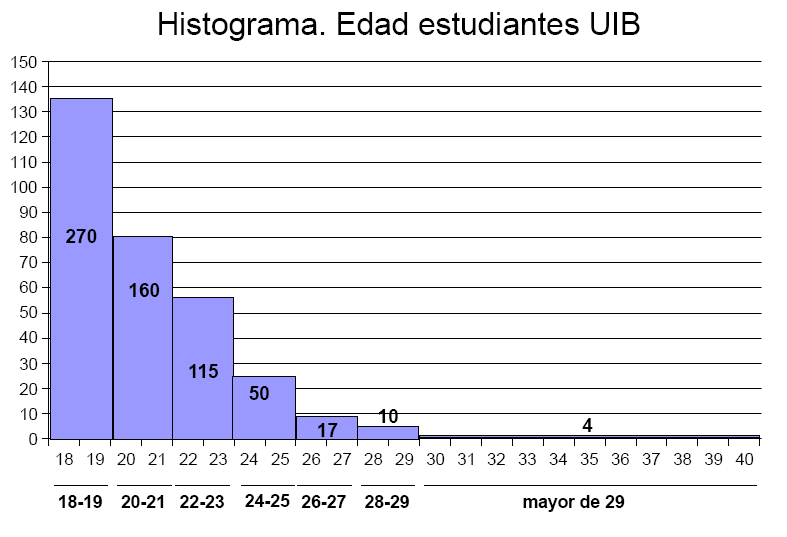
\includegraphics[width=12cm]{ejemplo2chis.png} 
\end{center}
\caption{Histograma de frecuencias absolutas de la tabla \ref{tabla2c}}
\label{tabla2chis}
\end{figure}

El valor que se muestra en el interior de las barras de los histogramas 
de las figuras \ref{tabla2his} y \ref{tabla2chis} es la frecuencia absoluta
de cada intervalo y es igual a la anchura del intervalo multiplicada por la
altura de la barra. Por ejemplo, para la segunda barra del histograma
de la figura \ref{tabla2his}, el valor de frecuencia es 160 y la anchura del
intervalo [20, 21] es 2, por este motivo la altura de la barra es 80 
($160=2 \times 80$). 

La comparaci\'on de estos histogramas con los diagramas de barras mostrados
en las figuras \ref{tabla2bar}, \ref{tabla2bbar} y \ref{tabla2cbar} nos permiten 
observar las principales diferencias entre ambas representaciones:
\begin{enumerate}
\item En los histogramas, el \'area y no la altura de las barras es proporcional a la frecuencia representada.
Esto significa que si dos intervalos tienen la misma frecuencia pero uno de ellos es mayor que el otro
entonces su altura ser\'a inferior.
\item La barras no est\'an separadas por un espacio en blanco en los histogramas, al contrario que en 
los diagramas de barras.
\item Todos los valores entre el m\'inimo y el m\'aximo de la variable est\'an representados en el histograma,
pero no as\'i en el diagrama de barras. Esto se aprecia comparando las figuras
\ref{tabla2bbar} y \ref{tabla2cbar}. En este caso los valores de edad 31, 32, 33, 36, 37, 38
y 39 se representan en el histograma (con una barra de altura cero, que no se dibuja), en cambio
no aparecen en el diagrama de barras.
\end{enumerate}

Los intervalos de valores representados en el histograma pueden ser de anchuras diferentes, 
aunque es habitual que todos sean iguales (salvo para los valores extremos que suelen representarse
con intervalos de tipo ``mayor de'' o ``menor de'').

\item \textbf{Diagramas de tarta o pictogramas}.
En un diagrama de tarta se representan las proporciones o porcentajes mediante
sectores circulares de tama\~no proporcional al valor representado. Se suelen utilizar
para representar va\-ria\-bles nominales. Para el ejemplo sobre la inmigraci\'on por nacionalidades
obtendr\'iamos el diagrama de tarta que se muestra en la figura \ref{tabla1tar}.

\begin{figure}[htbp]
\begin{center}
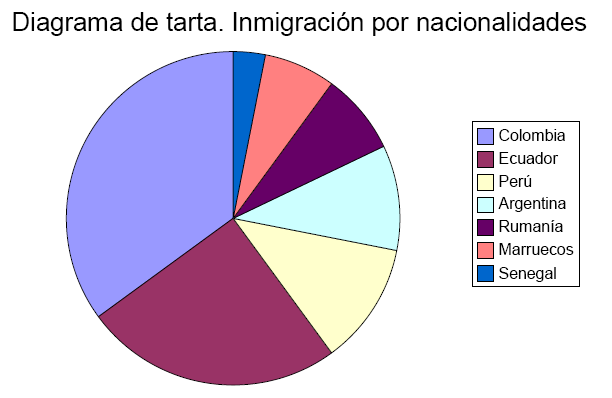
\includegraphics[width=8cm]{ejemplo1tar.png} 
\end{center}
\caption{Diagrama de tarta de porcentajes de la tabla \ref{tabla1}}
\label{tabla1tar}
\end{figure}


\item \textbf{Diagramas lineales}. En estos diagramas se unen mediante l\'ineas
una serie de puntos cuya coordenada horizontal representa el valor
de la variable y la vertical la frecuencia o porcentaje asociados al valor. 
Se utilizan para la des\-crip\-ci\'on de variables cuantitativas y son ideales
para apreciar las tendencias de los datos. Adem\'as, usando l\'ineas de distintos
colores o puntos de distintas formas permiten la representaci\'on conjunta
de datos de varias variables.
Cuando se emplean para representar frecuencias (absolutas, relativas o acumuladas)
se denominan \textbf{pol\'igonos de frecuencia} y cuando en el eje horizontal
se representan valores temporales (meses, a\~nos, etc.) se denominan 
\textbf{cronogramas}.

En la figura \ref{tabla2cline} se muestran los pol\'igonos de frecuencias absolutas
y acumuladas para el ejemplo sobre la edad de los estudiantes de la UIB de la tabla
\ref{tabla2c}. En la figura \ref{tabla5line} se muestra un ejemplo de cronograma.

\begin{figure}[htbp]
\begin{center}
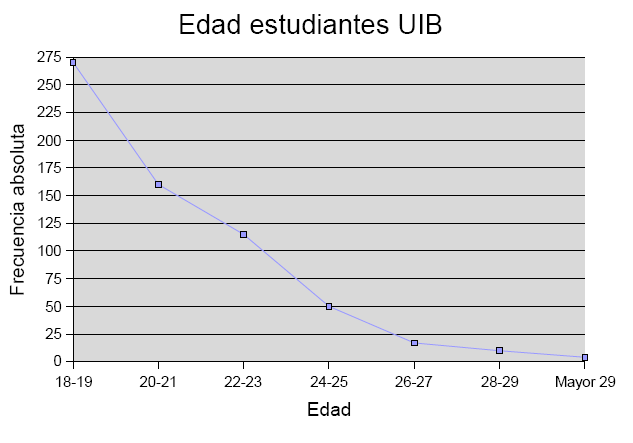
\includegraphics[width=10cm]{ejemplo2clinefabs.png} 
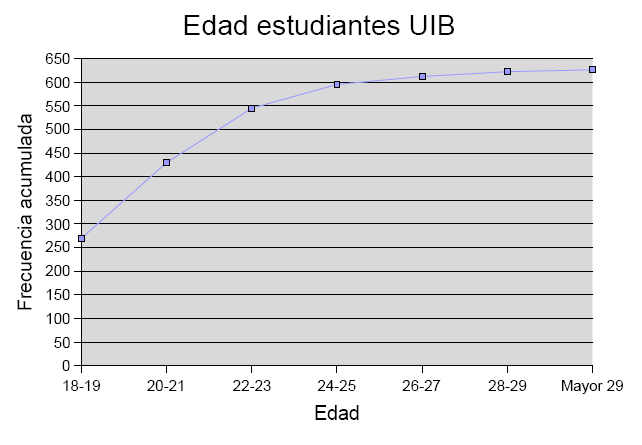
\includegraphics[width=10cm]{ejemplo2clinefacum.png} 
\end{center}
\caption{Ejemplo de la tabla \ref{tabla2c}. Arriba: pol\'igono de frecuencias absolutas. 
Abajo: pol\'igono de frecuencias acumuladas.}
\label{tabla2cline}
\end{figure}

\begin{figure}[htbp]
\begin{center}
\begin{tabular}{cc}
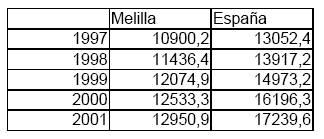
\includegraphics[width=6cm]{ejemplo5.png} &
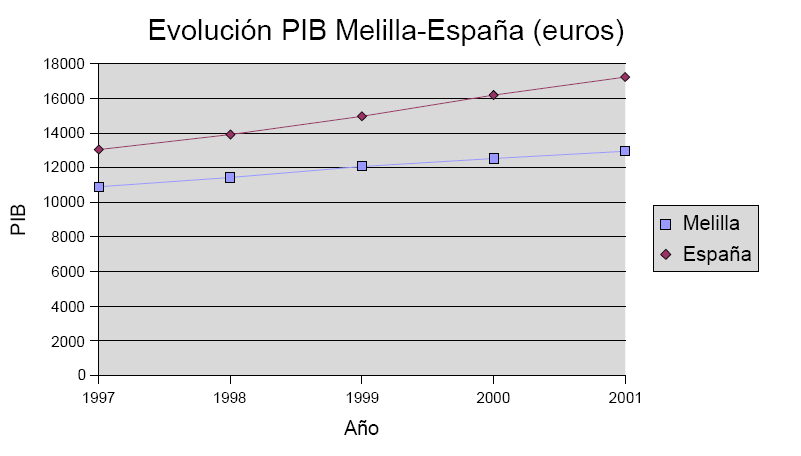
\includegraphics[width=9cm]{ejemplo5line.png}
\end{tabular} 
\end{center}
\caption{Izquierda: tabla de valores del PIB para Melilla y el conjunto de Espa\~na entre 1997 y 2001 (fuente INE).
Derecha: cronograma conjunto de los PIBs de Melilla y Espa�a}
\label{tabla5line}
\end{figure}


\section{Tablas y gr\'aficas estad\'isticas con ordenador}
\label{sectabgraford}
El c\'alculo de tablas de frecuencias y porcentajes as\'i como su representaci\'on gr\'afica
puede realizarse de manera sencilla con la ayuda de herramientas inform\'aticas.
Estudios estad\'isticos simples pueden rea\-li\-zar\-se mediante hojas de c\'alculo
(tipo Microsoft Excel o OpenOffice Calc). An\'alisis m\'as complejos requieren el uso de he\-rra\-mien\-tas
m\'as sofisticadas, como el software especializado en estad\'istica SPSS o R.

En esta secci\'on aprenderemos a obtener tablas y gr\'aficas mediante hojas de c\'alculo.
Utilizaremos el programa OpenOffice Calc, que es la versi\'on de software libre 
de hoja de c�lculo. El programa puede obtenerse de forma gratuita de \url{http://es.openoffice.org/}
y se instala f\'acilmente en cualquier sistema operativo. La versi\'on utilizada en 
los siguientes ejemplos es la 3.0.


%Consideremos el siguiente ejemplo, para el cual calcularemos las tablas de frecuencias
%y porcentajes, diagrama de barras, histograma, diagrama de tarta y pol\'igono de frecuencias.

\vskip 0.3 cm
\noindent
\textbf{Ejemplo 1}

Consideramos los siguientes datos obtenidos de la web del
Instituto Nacional de Estad�stica. Calcularemos la tabla de frecuencias
y porcentajes y haremos varias representaciones gr�ficas.

\begin{center}
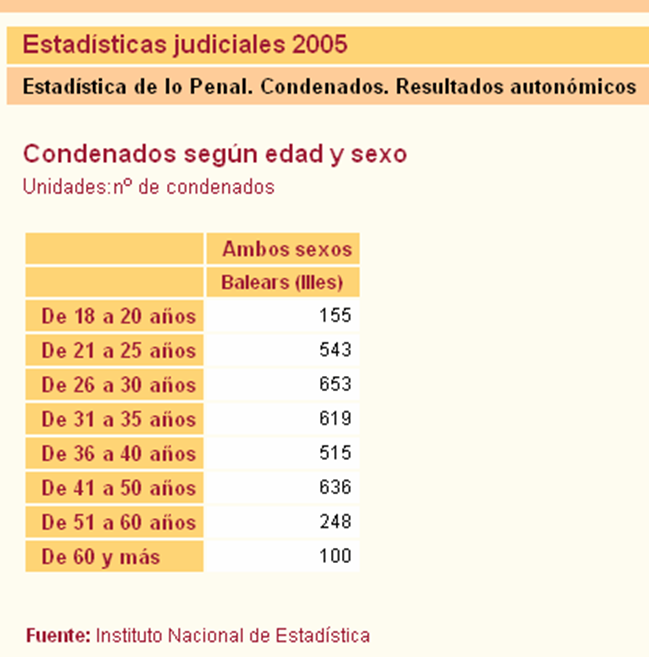
\includegraphics[width=10cm, height=7cm]{penalbalearsedad.png}
\end{center}

Los pasos a seguir para calcular las tablas de frecuencias
y porcentajes son los siguientes:

\begin{enumerate}
\item Abrir la aplicaci\'on OpenOffice Calc desde el men\'u de inicio de Windows:

\textit{Inicio:Todos los programas:OpenOffice.org:OpenOffice.org Calc}

Se abrir\'a una ventana como la que se muestra en la figura \ref{calcinicio}.

\begin{figure}[htbp]
\begin{center}
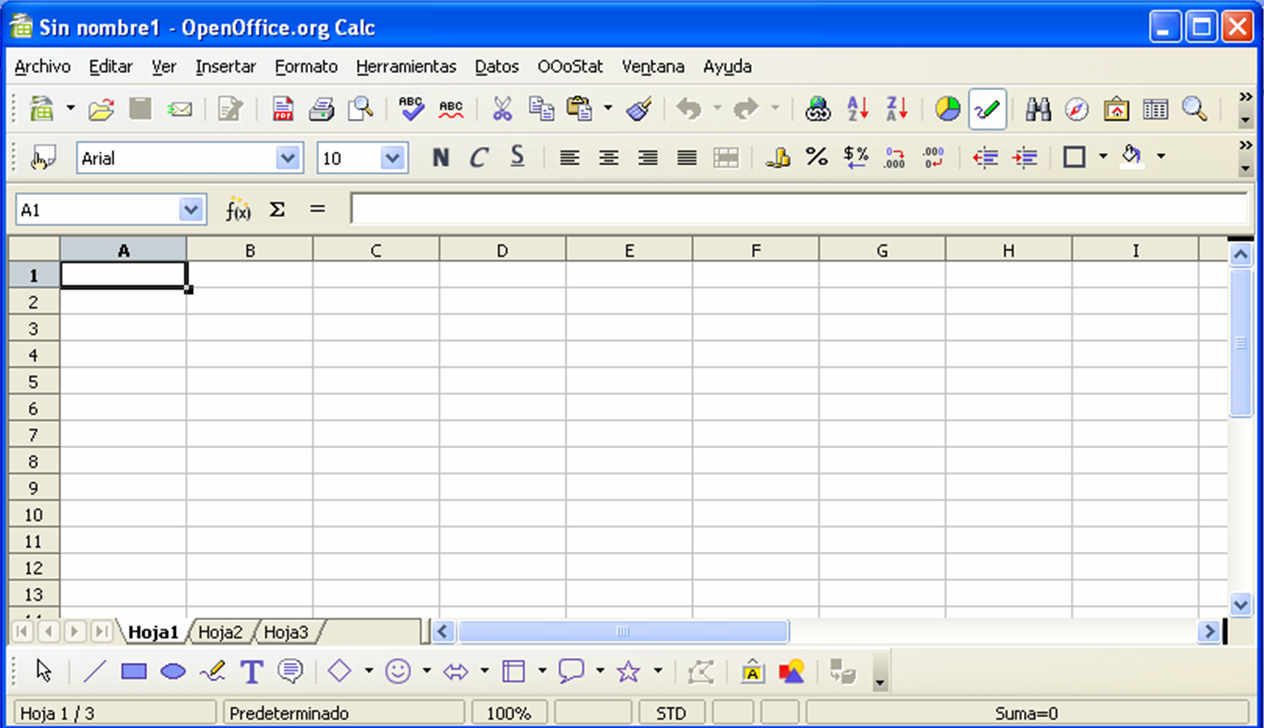
\includegraphics[width=15cm]{calcinicio.png}
\end{center}
\caption{Ventana de inicio de OpenOffice Calc}
\label{calcinicio}
\end{figure}

\item Para introducir los datos del problema nos situamos sobre la casilla $A1$ (columna $A$, fila $1$)
movi\'endonos con el cursor del rat\'on y escribimos en ella el t\'itulo de la tabla: 
\textit{Condenados Illes Balears por edad (a\~no 2005)}. La fila 2 la dejamos en blanco
para facilitar la lectura de la tabla. 

A continuaci\'on escribimos en la casilla $A3$ 
\textit{Edad (a\~nos)}, y en las
posiciones inferiores de la misma columna: $18-20$, $21-25$, $\cdots$, $51-60$,
\textit{m\'as de $60$}. Para desplazarnos de una casilla a la siguiente podemos utilizar el
rat\'on, las flechas del teclado o la tecla \textit{Tab}. 

Repetiremos la operaci\'on en la columna $B$. En la casilla $B3$ escribiremos \textit{$N^{o}$ condenados}
y en las casillas inferiores: $155$, $543$, $\cdots$, $100$.

Si en alg\'un momento deseamos rectificar alguno de los datos introducidos deberemos hacer doble clic
sobre la casilla correspondiente y reintroducir el valor.

Despu\'es de este paso la hoja de c\'alculo tendr\'a el aspecto que se muestra en la figura 
\ref{calcdatosini}.

\begin{figure}[htbp]
\begin{center}
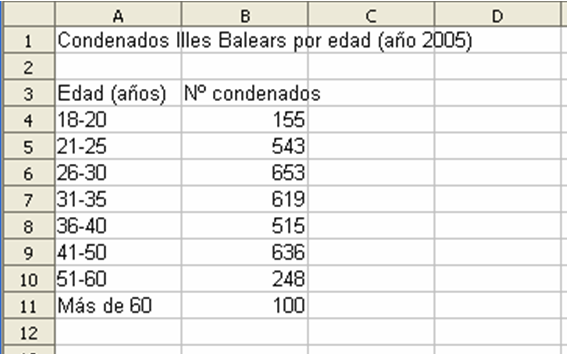
\includegraphics[width=7cm]{calcdatosini.png}
\end{center}
\caption{Hoja de c\'alculo tr\'as la introducci\'on de los datos del ejemplo 1}
\label{calcdatosini}
\end{figure}


\item Los valores de la columna B ($n^{o}$ condenados) son las frecuencias
absolutas de la variable \textit{Edad}. Deseamos calcular las frecuencias 
relativas y los porcentajes. Adem\'as, como la variable \textit{Edad}
es cuantitativa podemos calcular tambi\'en las frecuencias y porcentajes 
acumulados.

Empezamos por dar nombre a las columnas que mostrar\'an los valores 
calculados. Nos situamos sobre la casilla $C3$ y escribimos 
\textit{Frecuencia relativa}. Utilizando la tecla \textit{Tab} o el rat\'on 
nos des\-pla\-za\-re\-mos a la siguiente casilla de la misma fila (casilla $D4$)
y escribiremos \textit{Porcentaje}. Repitiendo el proceso escribiremos
en las casillas $E5$ a $H5$ los valores: \textit{Frecuencia absoluta acumulada},
\textit{Frecuencia relativa acumulada} y \textit{Porcentaje acumulado}.

Si el tama\~no del texto escrito es mayor que la anchura de la columna
el texto se sobreescribir\'a sobre las columnas vecinas. Para evitarlo
podemos aumentar la anchura de las columna situ\'andonos sobre las l\'ineas
que separan las letras de las columnas 

\begin{minipage}{5cm}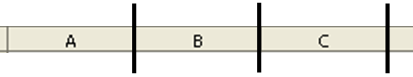
\includegraphics[width=5cm]{columnwidth.png}\end{minipage} 

y des\-pla\-z\'an\-do\-las con el cursor. 

Tambi\'en podemos ajustar el texto autom\'aticamente
al tama\~no de la columna situ\'andonos sobre la columna a modificar y 
siguiendo los siguientes pasos: acceder a la opci\'on \textit{Formato}
del men\'u principal, hacer clic sobre la opci\'on \textit{Celdas...},
se abrir\'a una nueva ventana en la que seleccionaremos la pesta\~na 
\textit{Alineaci\'on} y haremos clic sobre la opci\'on 
\textit{Ajustar texto autom\'aticamente} dentro del campo \textit{Propiedades}.

Tras estos ajustes la fila 3 de la hoja de c\'alculo contiene los si\-guien\-tes
valores:

\begin{center}
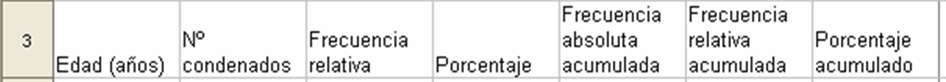
\includegraphics[width=12cm]{calcfila3.png}
\end{center}

\item Calcularemos primero la suma de los valores de frecuencias absolutas,
es decir, el n\'umero total de condenados. Escribiremos este valor al final
de la columna $B$ (casilla $B12$). Para ello nos situaremos sobre esta casilla,
escribiremos \verb@=SUMA(B4:B11)@ y pulsaremos la tecla \textit{Enter}.
El valor $3469$ se mostrar\'a en la casilla. La funci\'on \verb@SUMA@ es una 
funci\'on de Calc que permite sumar los valores de las casillas que se le
indican (en nuestro caso desde la casilla $B4$ hasta la $B11$).

\item Para calcular las frecuencias relativas debemos dividir las frecuencias
absolutas entre la suma de las frecuencias. Para ello nos si\-tua\-re\-mos sobre la
casilla $C4$, escribiremos \verb@=B4/$B$12@ y pulsaremos \textit{Enter}.
En la casilla aparece el valor $0,04$, resultado de dividir el valor de
las casillas $B4$ y $B12$. 

Podemos repetir la operaci\'on con el resto de las
casillas de la columna pero Calc ofrece una manera m\'as sencilla de hacer
estas operaciones. Basta situarnos con el cursor 
sobre la esquina inferior derecha de la
casilla $C4$, hacer clic con el bot\'on izquierdo del rat\'on y,
manteniendo el bot\'on pulsado, arrastrar el cursor hasta la casilla $C11$.
Al soltar el bot\'on aparecen en las casillas los valores calculados
(ver columna $C$ en la figura \ref{calctablafinal}), ya
que Calc reescribe autom\'aticamente la f\'ormula de la primera casilla
para adaptarla a las casillas seleccionadas.

%Los valores del resto de columnas se calculan de manera similar.

\item Los porcentajes se obtienen multiplicando las frecuencias relativas por
$100$. Para ello nos situamos sobre la casilla $D4$, escribimos \verb@=C4*100@
y pulsamos \textit{Enter}.
A continuaci\'on nos situamos con el cursor en la esquina inferior derecha 
de la casilla y, manteniendo el bot\'on izquierdo del rat\'on pulsado, arrastramos
el cursor hasta la casilla $D11$. Al soltar el bot\'on los resultados se escriben 
en las casillas correspondientes (ver columna $D$ en la figura \ref{calctablafinal}).

\item Las frecuencias absolutas acumuladas se calculan sumando a la frecuencia 
absoluta del valor considerado las frecuencias absolutas de los valores anteriores.
La frecuencia absoluta acumulada del primer valor ($18-20$) es igual a su
frecuencia absoluta, por lo que en la casilla $E4$ escribimos \verb@=B4@ y pulsamos
\textit{Enter}. En la casilla siguiente, $E5$, escribimos \verb@=E4+B5@ y pulsamos
\textit{Enter}. Las restantes casillas se calcular\'an autom\'aticamente si 
situamos el cursor en la esquina inferior derecha 
de la casilla $E5$ y, manteniendo el bot\'on izquierdo del rat\'on pulsado, arrastramos
el cursor hasta la casilla $E11$. Al soltar el bot\'on se muestran los valores calculados
(ver columna $E$ en la figura \ref{calctablafinal}).

\item Las frecuencias relativas acumuladas se calculan dividiendo las frecuencias
absolutas acumuladas entre la frecuencia absoluta total. Para ello escribimos en la
casilla $F4$ \verb@=E4/$B$12@ y pulsamos \textit{Enter}. 
Repitiendo el procedimiento explicado en los casos anteriores extendemos el c\'alculo
hasta la casilla $F11$ (el resultado se muestra en la columna $F$ en la figura \ref{calctablafinal}).

\item Finalmente, los porcentajes acumulados se obtienen multiplicando por $100$
las frecuencias relativas acumuladas. Para ello escribimos \verb@=F4*100@ y pulsamos
\textit{Enter} en la casilla $G4$. 
Repitiendo el procedimiento explicado en los casos anteriores extendemos el c\'alculo
hasta la casilla $G11$.

El tabla final obtenida se muestra en la figura \ref{calctablafinal}.

\begin{figure}[htbp]
\begin{center}
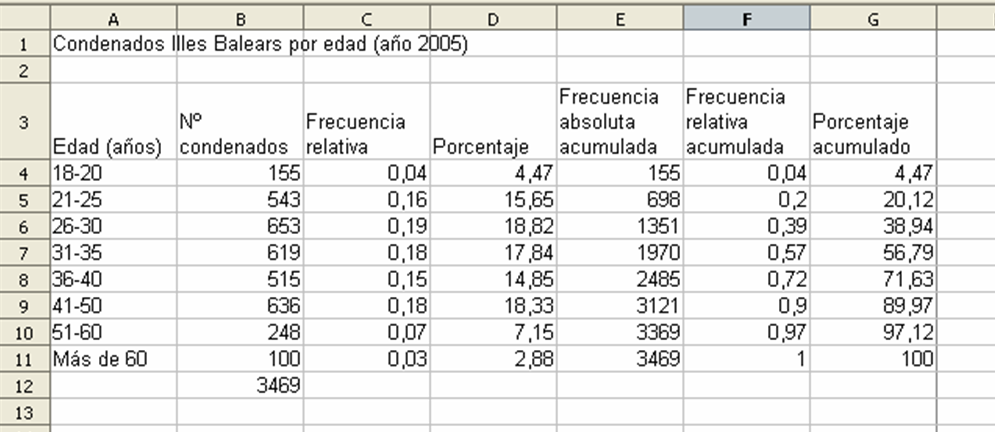
\includegraphics[width=12cm]{calctablafinal.png}
\end{center}
\caption{Frecuencias y porcentajes obtenidos a partir de los datos del ejemplo 1}
\label{calctablafinal}
\end{figure}

 
\item Podemos imprimir la tabla calculada o guardarla como un fichero .pdf
para su posterior impresi\'on
utilizando los iconos 
\begin{minipage}{0.5cm} 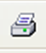
\includegraphics[width=0.5cm]{iconoprint.png}\end{minipage} 
 y  
\begin{minipage}{0.5cm} 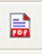
\includegraphics[width=0.5cm]{iconopdf.png}\end{minipage} 
respectivamente, del men\'u de Calc.

En todo caso, la visualizaci\'on de la tabla mejora si separamos las filas 
y las columnas mediante l\'ineas. Para ello, antes de imprimir o guardar el fichero
seleccionaremos todas las casillas de la tabla situ\'andonos sobre la 
casilla $A3$ y, manteniendo pulsado el bot\'on izquierdo del rat\'on, arrastrando el
cursor hasta la casilla $G12$. A continuaci\'on accederemos a la opci\'on \textit{Formato}
del men\'u principal, haremos clic sobre la opci\'on \textit{Celdas...},
se abrir\'a una nueva ventana en la que seleccionaremos la pesta\~na 
\textit{Borde} y haremos clic sobre el icono
\begin{minipage}{0.5cm} 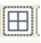
\includegraphics[width=0.5cm]{iconobordes.png}\end{minipage} .

Si imprimimos la tabla o visualizamos el fichero .pdf en la pantalla obtendremos el 
resultado de la figura \ref{calctablafinalpdf}:

\begin{figure}[htbp]
\begin{center}
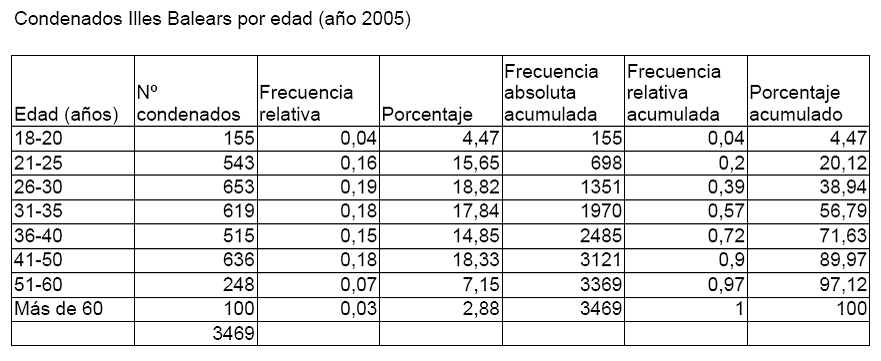
\includegraphics[width=12cm]{calctablafinalpdf.png}
\end{center}
\caption{Tabla final del ejemplo 1}
\label{calctablafinalpdf}
\end{figure}

La tabla anterior puede incluirse f\'acilmente en informes escritos con Microsoft Word o 
OpenOffice Writer. Para ello seleccionaremos con el cursor todas las casillas que componen
la tabla y utilizaremos la combinaci\'on de teclas \textit{Ctrl+C}. La tabla queda co\-pia\-da
en el portapapeles de Windows y puede ser pegada en otros documentos mediante la combinaci\'on
de teclas \textit{Ctrl+V}.


\end{enumerate}

\vskip 0.3 cm
A continuaci\'on explicamos como representar gr\'aficamente los valores calculados

\begin{enumerate}
\item \textbf{Creaci\'on de un diagrama de barras}.
Obtendremos en primer lugar un diagrama de barras que represente el n\'umero
de condenados en funci\'on de su edad. Los pasos a seguir son los siguientes:

\begin{enumerate}
\item Seleccionamos la opci\'on \textit{Insertar} del men\'u principal y 
hacemos clic sobre 
\begin{minipage}{2cm}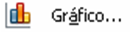
\includegraphics[width=2cm]{iconografico.png}\end{minipage}.
\item Se abrir\'a una ventana titulada \textit{Asistente de gr�ficos} 
(ver Figura \ref{ventana1barrasB}).
En primer lugar debemos seleccionar el tipo de diagrama, en nuestro caso un diagrama
de barras con texto, por lo que hacemos clic sobre el icono 
\begin{minipage}{1cm}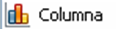
\includegraphics[width=1cm]{iconocolumna.png}\end{minipage}.
En la parte derecha de la ventana se elige una variante del diagrama de
barras, nosotros nos quedamos con la opci\'on por defecto (\textit{Normal})
y pulsamos \textit{Siguiente}.

\item Se muestra una nueva ventana donde seleccionaremos las casillas de datos a representar. 
Para ello escribiremos 

\verb@A3:A11;B3:B11@ en \textit{Rango de datos}.

Los datos de la primera columna seleccionada se representar\'an sobre el eje horizontal
y los de la segunda sobre el eje vertical. Haciendo clic sobre el bot\'on 
\textit{Siguiente} pasamos a la siguiente ventana (\textit{Series de datos}). Aplicamos
las opciones por defecto por lo que volvemos a pulsar \textit{Siguiente}.

\begin{figure}[htbp]
\begin{center}
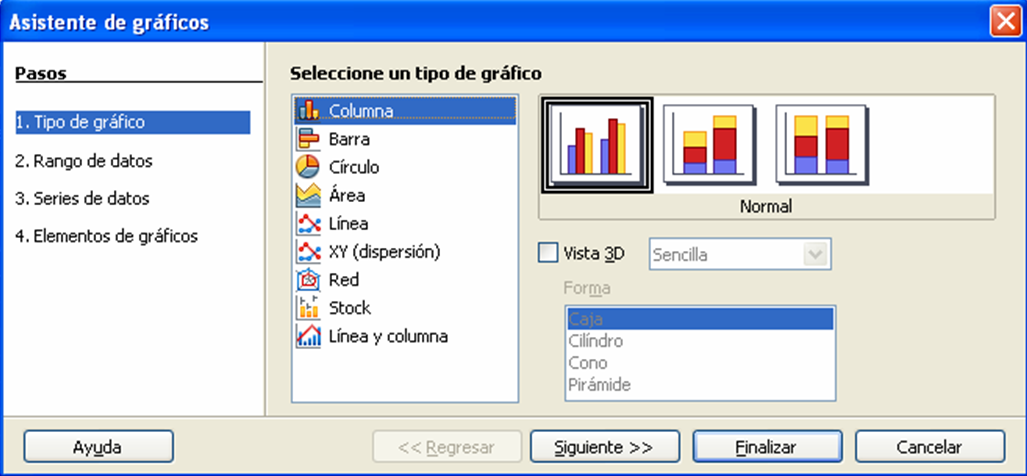
\includegraphics[width=12cm]{ventana1barrasB.png}
\end{center}
\caption{Inserci\'on de un diagrama de barras. Ventana inicial del \textit{Asistente de gr�ficos}}
\label{ventana1barrasB}
\end{figure}



\item En la \'ultima ventana debemos a�adir el texto de la gr\'afica.
Escribimos el \textit{T\'itulo del diagrama}: ``Condenados Illes Balears (a\~no 2005)'',
los t\'itulos de los ejes X e Y (``Edad'' y ``$N^o$ condenados'', respectivamente) y
desactivamos la opci\'on \textit{Mostrar leyenda}. 
%Los datos de la ventana se muestran en la figura \ref{ventana2barras}. 
Finalmente pulsamos el bot\'on \textit{Finalizar}.

El gr\'afico creado se muestra sobre la hoja de c\'alculo. Podemos variar su posici\'on
y tama\~no mediante el rat\'on. El resultado final se muestra en la figura \ref{calcbarrasej1}.

Al igual que para la tabla de frecuencias este diagrama puede imprimirse o bien guardarse
como un fichero .pdf. Adem\'as, haciendo clic sobre el mismo y utilizando la combinaci\'on
de teclas \textit{Ctrl+C} es posible copiarlo en el portapapales de Windows. De esta forma
puede ser pegado f\'acilmente (combinaci\'on de teclas \textit{Ctrl+V}) en un documento de 
Microsoft Word o OpenOffice Writer para la elaboraci\'on de un informe.

%\begin{figure}[htbp]
%\begin{center}
%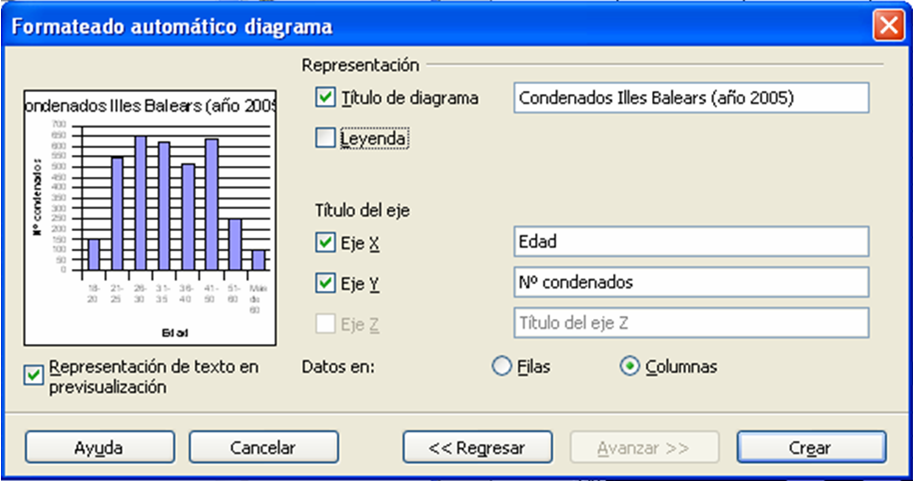
\includegraphics[width=12cm]{ventana2barras.png}
%\end{center}
%\caption{Inserci\'on de un diagrama de barras. Ventana final del proceso de formateado
%autom\'atico}
%\label{ventana2barras}
%\end{figure}

\begin{figure}[htbp]
\begin{center}
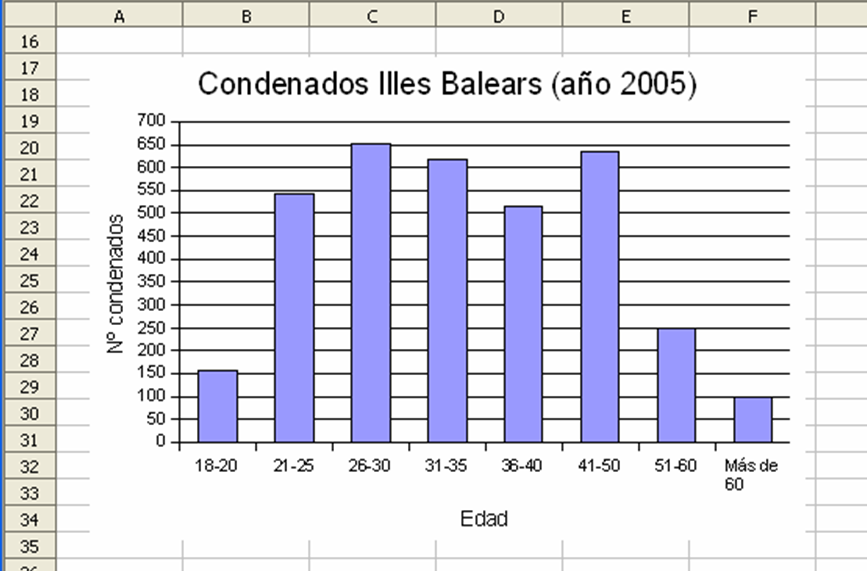
\includegraphics[width=9cm]{calcbarrasej1.png}
\end{center}
\caption{Diagrama de barras de frecuencias absolutas del ejemplo 1}
\label{calcbarrasej1}
\end{figure}

\end{enumerate}

\item \textbf{Creaci\'on de un diagrama de tarta}. Obtendremos a con\-ti\-nua\-ci\'on
un diagrama de tarta que represente los porcentajes de condenados para cada intervalo
de edad. Los pasos a seguir son pr\'acticamete id\'enticos a los del diagrama de barras,
con las si\-guien\-tes modificaciones
\begin{enumerate}
\item En la ventana inicial del \textit{Asistente de gr\'aficos}
seleccionamos el tipo de diagrama haciendo clic sobre el icono
\begin{minipage}{1cm}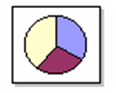
\includegraphics[width=1cm]{iconotarta.png}\end{minipage}
 (C\'irculo).
\item En la siguiente ventana el rango de datos es \verb@A3:A11;D3:D11@.
\item Una vez creado el diagrama es posible cambiar el tama\~no del texto de la leyenda
haciendo doble clic sobre el diagrama, seleccionando la opci\'on \textit{Formato}
del men\'u principal y a continuaci\'on la opci\'on \textit{Leyenda}. Aparece una nueva
ventana en la que hay que escoger la pesta\~na \textit{Caracteres} y el \textit{Tama\~no}
deseado. El resultado final se muestra en la figura \ref{calctartaej1}.

\begin{figure}[htbp]
\begin{center}
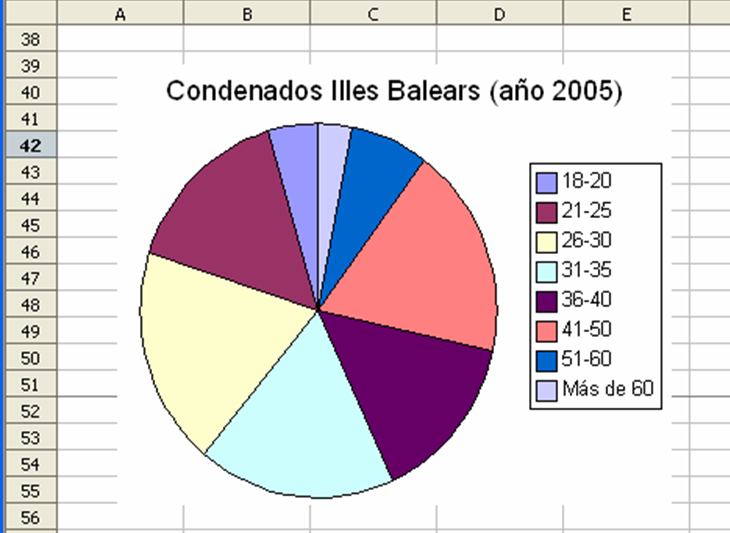
\includegraphics[width=9cm, height=5cm]{calctartaej1.png}
\end{center}
\caption{Diagrama de tarta de porcentajes del ejemplo 1}
\label{calctartaej1}
\end{figure}



\item Este diagrama puede ser imprimido o insertado en otro documento al igual que el
diagrama de barras.

\end{enumerate}

%\item \textbf{Creaci\'on de un diagrama de Pareto}. Explicamos a continuaci\'on c\'omo crear
%un diagrama de Pareto de frecuencias relativas y frecuencias relativas acumuladas.
%Los pasos a seguir son muy similares a los de los diagramas anteriores, con las siguientes
%modificaciones:
%\begin{enumerate}
%\item En la ventana inicial de \textit{Formateado autom\'atico diagrama} debemos
%seleccionar las casillas $A3$ hasta $A11$, $C3$ hasta $C11$ y $F3$ hasta $F11$.
%\item El tipo de diagrama a seleccionar es el de barras pero la variante a escoger
%es la representada con el icono 
%\begin{minipage}{1cm}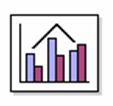
\includegraphics[width=1cm]{iconopareto.png}\end{minipage}.
%\item En la \'ultima ventana para el formateado del diagrama activamos la opci\'on
%\textit{Leyenda} y dejamos sin t\'itulo el eje Y. A continuaci\'on creamos el diagrama.
%
%Mediante el cursor podemos cambiar de tama\~no y posici\'on el gr\'afico creado
%y podemos aumentar la talla del texto de la leyenda tal como se ha explicado
%para el diagrama de tarta. El resultado final se muestra en la figura \ref{calcparetoej1}.
%
%\begin{figure}[htbp]
%\begin{center}
%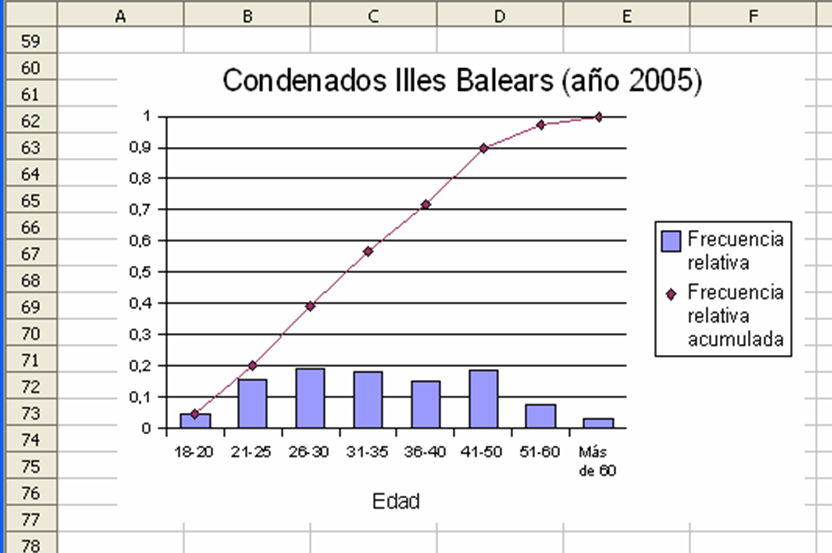
\includegraphics[width=9cm]{calcparetoej1.png}
%\end{center}
%\caption{Diagrama de Pareto de frecuencias relativas del ejemplo 1}
%\label{calcparetoej1}
%\end{figure}
%
%\end{enumerate}

\end{enumerate}

\newpage
\noindent
\textbf{Ejemplo 2} 

En este ejemplo aprenderemos a crear un diagrama de barras dobles a partir de los siguientes
datos sobre poblaci\'on reclusa menor de edad en Baleares:

\vskip 0.2 cm
\begin{center}
\begin{tabular}{|c|c|c|}
\hline
Edad (a\~nos) & Var\'on & Mujer \\ \hline
14 & 62 & 6 \\ \hline
15 & 78 & 10 \\ \hline
16 & 134 & 21 \\ \hline
17 & 332 & 29 \\ \hline
\end{tabular}
\end{center}

\begin{enumerate}
\item Introducimos los datos en una hoja de c\'alculo tal como se ha explicado 
para el ejemplo 1. Supongamos por ejemplo que los datos de \textit{Edad}
ocupan las casillas $A4$ a $A7$, los de \textit{Var\'on} las casillas $B4$ a $B7$ y los 
de \textit{Mujer} de $C4$ a $C7$ (las casillas $A3$, $B3$ y $C3$ contienen los t�tulos de
las columnas). 

\item Seguimos los pasos explicados para la creaci\'on de diagramas de barras en el
ejemplo 1 pero seleccionando ahora las tres columnas de datos (rango de valores 
\verb@A3:A7;B3:B7;C3:C7@).
Las opciones a elegir son las mismas que en el caso del ejemplo 1 con la diferencia
de que en la \'ultima ventana seleccionamos la opci\'on \textit{Mostrar leyenda} y que los t\'itulos
del diagrama y los ejes X e Y son, respectivamente: ``Poblaci\'on reclusa menor de edad
en Baleares'', ``Edad'' y ``$N^o$ reclusos''.

Al pulsar sobre el bot\'on \textit{Finalizar} obtenemos el resultado que se muestra
en la figura \ref{calcbarrasej2}.

\begin{figure}[htbp]
\begin{center}
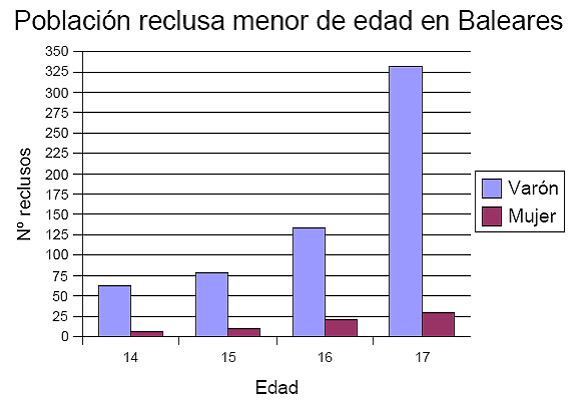
\includegraphics[width=9cm]{calcbarrasej2.png}
\end{center}
\caption{Diagrama de barras dobles del ejemplo 2}
\label{calcbarrasej2}
\end{figure}

\end{enumerate}


\vskip 0.5 cm
\noindent
\textbf{Ejemplo 3} 

En este ejemplo mostramos c\'omo calcular un histograma de frecuencias
absolutas a partir de los datos siguientes sobre el peso de un grupo de 
personas:

\vskip 0.2 cm
\begin{center}
\begin{tabular}{|c|c|}
\hline
Peso (Kg) & Frecuencia absoluta \\ \hline
45-49 & 20 \\ \hline
50-54 & 35 \\ \hline
55-59 & 40 \\ \hline
60-64 & 55 \\ \hline
65-69 & 45 \\ \hline
70-74 & 50 \\ \hline
75-79 & 35 \\ \hline
80-84 & 30 \\ \hline
85-89 & 25 \\ \hline
90-94 & 15 \\ \hline
95-99 & 5 \\ \hline
\end{tabular}
\end{center}

\begin{enumerate}
\item En primer lugar creamos un documento OpenOffice Calc con
los datos de la tabla anterior, tal como se ha explicado en el
ejemplo 1. Supongamos que los datos sobre \textit{Peso}
ocupan las casillas $A4$ a $A14$ y los de frecuencia absoluta las 
casillas $B4$ a $B14$ (ver figura \ref{calctabej3}).

\item OpenOffice Calc no proporciona ninguna herramienta para la
creaci\'on autom\'atica de histogramas en un caso general. S\'olo en
el caso de que todos los intervalos de valores sean de la misma amplitud
(como en este ejemplo) es posible crear un histograma de manera sencilla.

En el caso del ejemplo todos los intervalos son de longitud $5$ y podemos 
representar el histograma como un diagrama de barras modificado.
En primer lugar debemos calcular la altura de las barras. 

Sabemos que el \'area
de las barras del histograma es igual al valor re\-pre\-sen\-tado (en este caso 
la frecuencia absoluta). Por ejemplo, la primera barra debe tener \'area $20$,
como su anchura es $5$ su altura deber\'a ser $\displaystyle \frac{20}{5} =4$.
Razonando de la misma manera podemos calcular el resto de alturas.
Podemos hacerlo de forma autom\'atica con Calc: escribimos en la casilla $C4$
\verb@=B4/5@, pulsamos \textit{Enter} y a continuaci\'on extendemos el c\'alculo
hasta la casilla $C14$ utilizando el m\'etodo explicado en el ejemplo 1. Al final de
esta operaci\'on en la columna $C$ aparecen los valores de altura calculados
(ver figura \ref{calctabej3}).

\begin{figure}[htbp]
\begin{center}
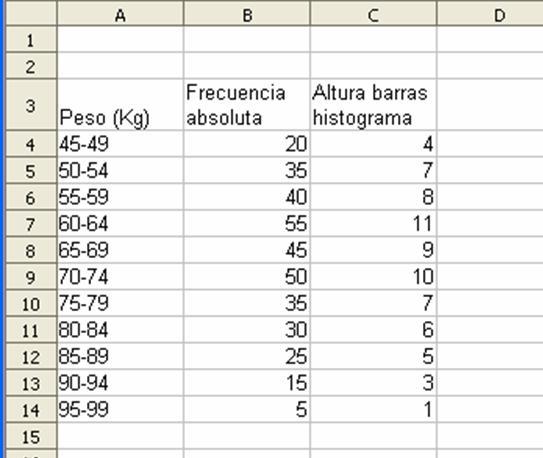
\includegraphics[width=6cm]{calctabej3.png}
\end{center}
\caption{Tabla de datos del ejemplo 3}
\label{calctabej3}
\end{figure}

\item Ahora el histograma se puede calcular como un diagrama de ba\-rras. Seguimos
el procedimiento descrito para el ejemplo 3 seleccionando las casillas $A3$ a $A14$
y $C3$ a $C14$ en el rango de datos. 
Los t\'itulos del diagrama y del eje X son, respectivamente, ``Histograma
pesos'' y ``Pesos (Kg)'' y la opci\'on \textit{Mostrar leyenda} no se selecciona.

Al crear el diagrama obtenemos un diagrama de barras con las barras separadas.
Para unir las barras y darle la forma t\'ipica de un histograma debemos hacer 
doble clic sobre una de las barras del diagrama hasta que aparece la ventana
que se muestra en la figura \ref{ventana1hist}. Escogemos la pesta\~na \textit{Opciones}
y ponemos a $0\%$ el valor de \textit{Espacio} en la opci\'on \textit{Configuraci\'on}.
Al pulsar sobre el bot\'on \textit{Aceptar} de esta ventana obtenemos un histograma
como el que se muestra en la figura \ref{calchistej3}.

\begin{figure}[htbp]
\begin{center}
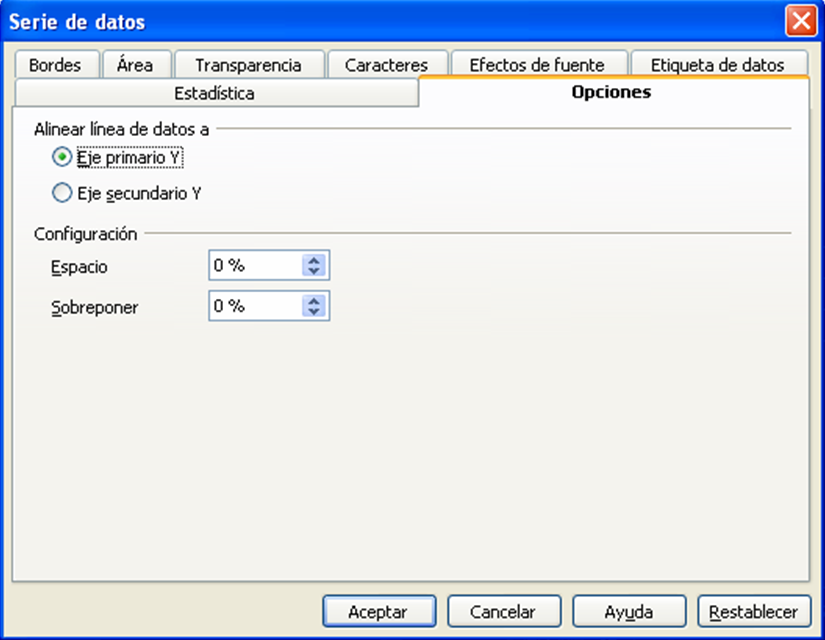
\includegraphics[width=10cm]{ventana1hist.png}
\end{center}
\caption{Ventana de di\'alogo para ajustar la anchura de las barras del diagrama de barras}
\label{ventana1hist}
\end{figure}

\begin{figure}[htbp]
\begin{center}
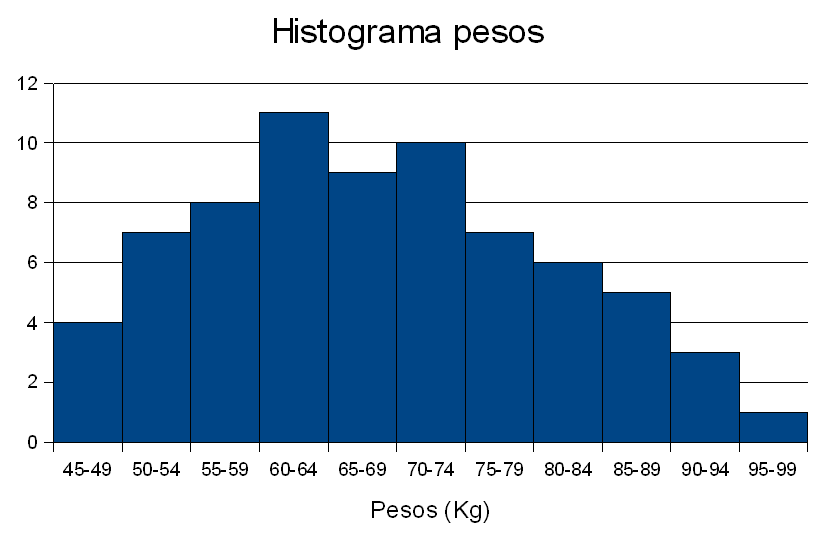
\includegraphics[width=10cm]{calchistej3.png}
\end{center}
\caption{Histograma del ejemplo 3}
\label{calchistej3}
\end{figure}


\end{enumerate}


\vskip 0.5 cm
\noindent
\textbf{Ejemplo 4}

En este ejemplo mostramos c\'omo crear un diagrama lineal que representa 
la evoluci\'on del PIB espa\~nol (en miles de millones de dolares) 
desde 1992 hasta 2007. Los datos proceden del Fondo Monetario Internacional.

\vskip 0.2 cm
\begin{center}
\begin{tabular}{|c|c|}
\hline
A\~no & PIB \\ \hline
1992 & 612 \\ \hline
1993 & 513 \\ \hline
1994 & 515 \\ \hline
1995 & 597 \\ \hline
1996 & 622 \\ \hline
1997 & 573 \\ \hline
1998 & 601 \\ \hline
1999 & 618 \\ \hline
\end{tabular}
$\qquad$
\begin{tabular}{|c|c|}
\hline
A\~no & PIB \\ \hline
2000 & 582 \\ \hline
2001 & 609 \\ \hline
2002 & 688 \\ \hline
2003 & 885 \\ \hline
2004 & 1045 \\ \hline
2005 & 1131 \\ \hline
2006 & 1231 \\ \hline
2007 & 1414 \\ \hline
\end{tabular}
\end{center}

\begin{enumerate}
\item En primer lugar creamos un documento OpenOffice Calc con
los datos de la tabla anterior, tal como se ha explicado en el
ejemplo 1. Supongamos que los datos sobre \textit{A\~nos}
ocupan las casillas $A4$ a $A19$ y los de PIB las 
casillas $B4$ a $B19$ (en $A3$ y $B3$ se encuentran los nombres
de las columnas).

\item Creamos un diagrama siguiendo el procedimiento explicado en 
anteriores ejemplos. Las casillas de datos a seleccionar son de $A3$ a $A19$
y $B3$ a $B19$.

Seleccionamos el tipo de diagrama representado por el icono
\begin{minipage}{1cm}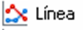
\includegraphics[width=1cm]{iconolineal.png}\end{minipage}
y la variante representada por el icono
\begin{minipage}{1cm}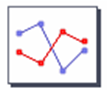
\includegraphics[width=1cm]{iconolinealpunts.png}\end{minipage}.

No seleccionamos la opci\'on de \textit{Mostrar leyenda} y los t\'itulos del diagrama y los
ejes X e Y son, respectivamente, ``Evoluci\'on PIB de Espa\~na'', ``A\~no'' y 
``PIB (miles millones dolares)''. La gr\'afica obtenida se muestra en la figura
\ref{calclinealej4}.


\begin{figure}[htbp]
\begin{center}
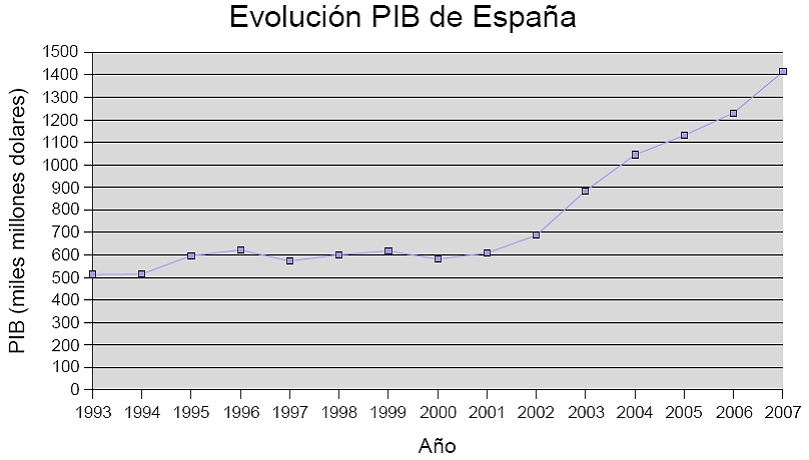
\includegraphics[width=12cm]{calclinealej4.png}
\end{center}
\caption{Diagrama lineal del ejemplo 4}
\label{calclinealej4}
\end{figure}

\end{enumerate}

\vskip 0.5 cm
\noindent
\textbf{Ejemplo 5}

En todos los ejemplos anteriores hemos partido de datos de frecuencias
absolutas a partir de las cuales hemos calculado frecuencias acumuladas,
porcentajes, etc. Es habitual sin embargo disponer de datos \textit{en bruto}
que deben organizarse primero en tablas de frecuencias absolutas antes
de realizar cualquier otro c\'alculo.
En este \'ultimo ejemplo explicamos c\'omo organizar este tipo de datos.

Partimos de los datos que se muestran en el siguiente gr\'afico (fuente LFP):
\vskip 0.2 cm
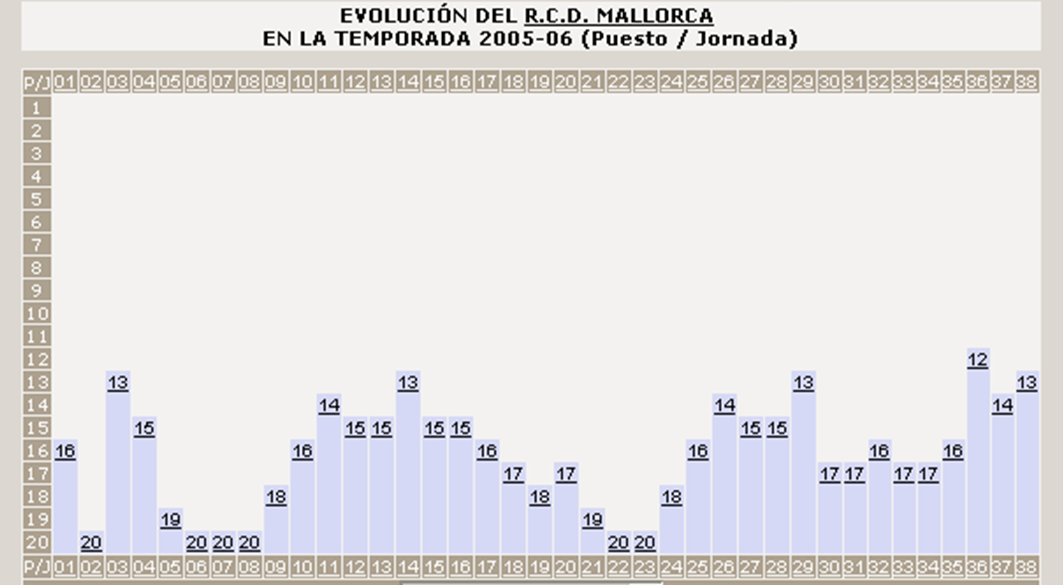
\includegraphics[width=13cm]{ejemplo5T2.png}

Para la variable ``clasificaci\'on del RCD Mallorca
durante la temporada 2005-2006'' deseamos calcular las frecuencias absolutas
y acumuladas. Los pasos a seguir son los siguientes:

\begin{enumerate}
\item Creamos un documento OpenOffice Calc y escribimos en la primera columna 
los datos \textit{brutos} del gr\'afico. Los datos ocupan las casillas $A1$ a $A38$.
El resultado se muestra en la figura 
\ref{calc1ej5}.

\begin{figure}[htbp]
\begin{center}
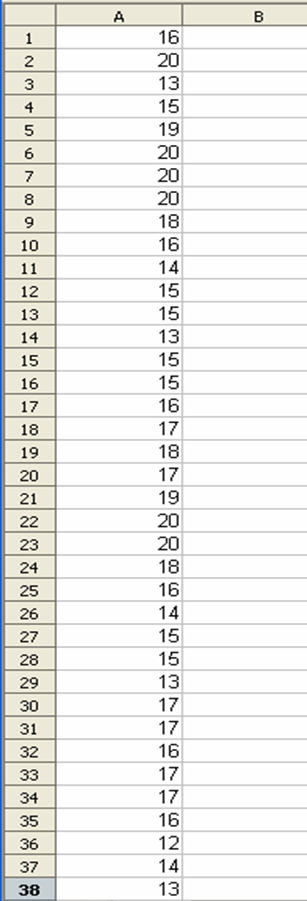
\includegraphics[width=3cm]{calc1ej5.png}
$\qquad \qquad$
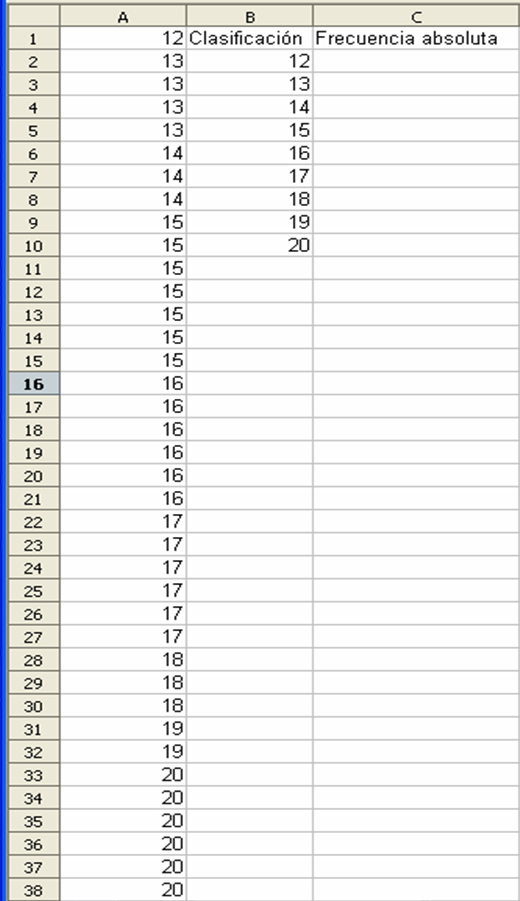
\includegraphics[width=7cm]{calc2ej5.png}
\end{center}
\caption{Izquierda: documento OpenOffice Calc con los datos \textit{en bruto} del ejemplo 5 (paso 1).
Derecha: documento preparado para el c\'alculo de las frecuencias absolutas (paso 2)}
\label{calc1ej5}
\end{figure}

\item A continuaci\'on creamos dos nuevas columnas en el documento 
(por ejemplo, las columnas $B$ y $C$).
En la parte superior de la primera columna escribimos el nombre de la variable 
(``Clasificaci\'on'') y a continuaci\'on escribimos, en orden creciente, 
los distintos valores que toma la variable. En la parte superior de la segunda columna
escribimos ``Frecuencia absoluta'', que calcularemos a continuaci\'on. 

%Para facilitar la tarea de escribir en orden creciente los distintos valores 
%de la variable podemos \textbf{ordenar} los valores \textit{brutos} del siguiente modo:
%\begin{enumerate}
%\item Seleccionamos las casillas A1 a A38 manteniendo el bot�n izquierdo del rat\'on pulsado.
%\item En el men\'u principal escogemos la opci\'on \textit{Datos}, y a continuaci\'on \textit{Ordenar...}
%\item Se abre una ventana en la que se definen los criterios de ordenaci\'on. En nuestro caso
%aceptamos la opciones por defecto: \textit{Ordenar seg\'un:  Columna A} y \textit{Ascendente}. Pulsamos
%\textit{Enter}.
%\item Los valores de las casillas seleccionadas se ordenan de menor a mayor. Ahora es sencillo
%ver qu� valores toma la variable y escribirlos de forma ordenada en la columna C.
%\end{enumerate}

Para facilitar la tarea de escribir en orden creciente los distintos valores 
de la variable podemos \textbf{ordenar} los valores \textit{brutos} del siguiente modo:
\begin{enumerate}
\item Seleccionamos las casillas $A1$ a $A38$ manteniendo el bot�n izquierdo del rat\'on pulsado.
\item Pulsamos el icono 
\begin{minipage}{1cm}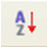
\includegraphics[width=1cm]{iconoAZ.png} \end{minipage}. Los valores se ordenan
de menor a mayor. (Con la opci\'on 
\begin{minipage}{1cm}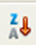
\includegraphics[width=1cm]{iconoZA.png}\end{minipage} 
los valores se ordenar\'ian de mayor a menor).

Ahora es sencillo ver qu� valores toma la variable y escribirlos de forma ordenada en la columna $C$.
\end{enumerate}


Al final de este paso el documento Calc tiene la forma que se muestra en la figura
\ref{calc1ej5}-derecha.

\item Para calcular las frecuencias absolutas nos situamos en la casilla $C2$, correspondiente
a la frecuencia absoluta del valor $12$. Escribimos 

\verb@=CONTAR.SI($A$1:$A$38;"="&B2)@
\footnote{La instrucci\'on \texttt{=CONTAR.SI($A$1:$A$38;``=''\&B2)} 
examina las columnas $A1$ a $A38$
y cuenta cu\'antas de ellas tienen un valor igual al de la casilla $B2$} 
y 
pulsamos \textit{Enter}. Un $1$ aparece escrito en la casilla, lo que significa que el valor $12$
aparece un \'unica vez en la lista de datos \textit{brutos} (su frecuencia absoluta es $1$).
Extendemos el c\'alculo a las casillas $C3$ a $C10$ del siguiente modo: 
situamos el cursor en la esquina inferior derecha 
de la casilla $C5$ y, manteniendo el bot\'on izquierdo del rat\'on pulsado, arrastramos
el cursor hasta la casilla $C10$. Al soltar el bot\'on se mostrar\'an los valores calculados.
Al final de este paso la hoja de c\'alculo tiene el aspecto que se muestra en la figura 
\ref{calc3ej5}-izquierda.


\begin{figure}[htbp]
\begin{center}
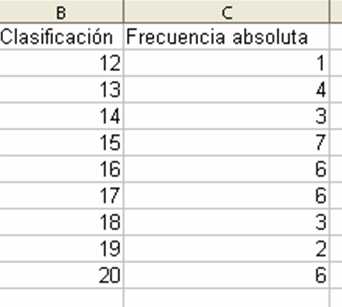
\includegraphics[width=4 cm]{calc3ej5.png}
$\qquad$
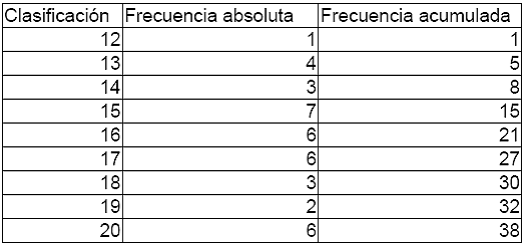
\includegraphics[width=9cm]{calc4ej5.png}
\end{center}
\caption{Izquierda: frecuencias absolutas del ejemplo 5 (paso 3). Derecha: tabla final.}
\label{calc3ej5}
\end{figure}

\item Las frecuencias acumuladas se calculan siguiendo el procedimiento explicado en
los ejemplos anteriores. La tabla final se muestra en la figura \ref{calc3ej5}.

%\begin{figure}[htbp]
%\begin{center}
%\includegraphics[width=10cm]{calc4ej5.png}
%\end{center}
%\label{calc4ej5}
%\caption{Tabla final del ejemplo 5}
%\end{figure}



\end{enumerate}








\clearpage

\section{Utilizaci\'on de la base de datos del INE}
\label{secINE}
El Instituto Nacional de Estad\'istica (INE) ofrece a trav\'es de su
p\'agina web gran cantidad de informaci\'on sobre distintos temas:
Educaci\'on, Cultura, Salud, Econom\'ia, Justicia, etc.
Los datos de los ejemplos de la secci\'on anterior se han obtenido 
de esta web. En esta secci\'on explicamos c�mo utilizar la base de datos
del INE.

Por ejemplo, supongamos que deseamos hacer un estudio sobre Educaci\'on.
Los pasos a seguir para obtener los datos del INE son los siguientes:
\begin{enumerate}
\item abrir en el navegador la direcci\'on \url{http://www.ine.es}
\item hacer clic sobre la opci\'on 
\begin{minipage}{4cm}\includegraphics[width=4cm]{inelogo.png}\end{minipage}
%\textit{INebase Toda la informaci\'on estad\'istica del INE}, 
que aparece a la izquierda de la p\'agina principal
\item las diferentes opciones de la base de datos se muestran en la nueva 
p\'agina (ver Figura \ref{opcionesine})

\begin{figure}[htbp]
\begin{center}
\includegraphics[width=14cm]{opcionesine.png}
\end{center}
\caption{Opciones de la base de datos del INE}
\label{opcionesine}
\end{figure}

\item para acceder a los datos sobre Educaci\'on hacemos clic sobre 
\textit{E\-du\-ca\-ci\'on} (bajo el ep\'igrafe \textit{Sociedad}) en el 
men\'u principal

\item en la nueva p\'agina se ofrecen varios estudios estad\'isticos 
relacionados con la educaci\'on.
Supongamos que deseamos conocer los datos sobre \textit{Gasto
p\'ublico en educaci\'on}, para haremos clic sobre este concepto.

%\begin{figure}[htbp]
%\begin{center}
%\includegraphics[width=16cm]{opcioneseduca.png}
%\end{center}
%\caption{Datos sobre educaci\'on en la base de datos del INE}
%\label{opcioneseduca}
%\end{figure}
% 
\item en la nueva p\'agina que se abre se explica en qu\'e consisten
los datos recopilados y se permite al usuario acceder a la 
informaci\'on de un a\~no en concreto. En el menu desplegable
que aparece al hacer clic sobre \textit{Seleccione un a\~no}
escogemos por ejemplo la opci\'on \textit{2004-2005}

\item se nos ofrecen varios tipos de datos (ver Figura \ref{becaseduca}).
Elegimos por ejemplo la opci\'on \textit{Becas e importe de las mismas por 
universidad en la que est� matriculado el becario, n�mero, entidad que las 
concede y tipo de beca}, bajo el ep\'igrafe \textit{Ense\~nanzas universitarias}

\begin{figure}[htbp]
\begin{center}
\includegraphics[width=13.5cm]{becaseduca.png}
\end{center}
\caption{Datos sobre gasto p\'ublico en educaci\'on en la base de datos del INE}
\label{becaseduca}
\end{figure}

\item la nueva p\'agina que se abre nos permite escoger los datos a mostrar y 
la manera de mostrarlos mediante una serie de menus (ver Figura \ref{becasmenus}).
Podemos seleccionar por ejemplo las universidades Aut\'onoma de Barcelona,
Complutense de Madrid, Illes Balears, P\'ublica de Navarra, Sevilla y Deusto.

Para ello haremos clic sobre las opciones 
del men\'u \textit{Universidad en la que est� matriculado el becario}, manteniendo
pulsada la tecla \textit{Ctrl}, lo que nos permitir\'a la selecci\'on simult\'anea 
de varias opciones.

A continuaci\'on seleccionaremos las opciones Becas e Importe en el men\'u 
\textit{N�\-me\-ro} (manteniendo pulsada la tecla \textit{Ctrl}), la opci\'on
Todas las Administraciones en el men\'u \textit{Entidad que las concede}
y Total en \textit{Tipo de beca}.

Finalmente elegiremos la forma de visualizar los datos. Podemos elegir qu\'e
variables se mostrar\'an por filas y cuales por columnas. Por defecto el men\'u
nos ofrece visualizar por filas la variable \textit{Universidad en la que est\'a
matriculado el becario} y por columnas el n\'umero de becas, la entidad que las
concede y el tipo. Aceptamos las opciones por defecto y ge\-ne\-ra\-mos el resultado
pulsando el bot\'on \begin{minipage}{3cm}\includegraphics[width=3cm]{consultselec.png}\end{minipage}.
Obtendremos el resultado que se muestra en la figura \ref{becastabla}

\begin{figure}[htbp]
\begin{center}
\includegraphics[width=13.5cm]{becasmenus.png}
\end{center}
\caption{Menus para la selecci\'on de datos sobre n\'umero de becas e importe de las
mismas en centros universitarios}
\label{becasmenus}
\end{figure}
 
\begin{figure}[htbp]
\begin{center}
\includegraphics[width=13.5cm]{becastabla.png}
\end{center}
\caption{Tabla de datos sobre n\'umero de becas e importe de las
mismas en centros universitarios}
\label{becastabla}
\end{figure}

\item la tabla obtenida se puede imprimir pulsando el icono 
\begin{minipage}{0.5cm}\includegraphics[width=0.5cm]{printselec.png}\end{minipage} de la p\'agina de resultados.
Tambi\'en se puede guardar en distintos formatos para ser utilizada
por distintos programas estad�sticos pulsando sobre el bot\'on
\begin{minipage}{3cm}\includegraphics[width=3cm]{saveselec.png}\end{minipage}.

Nosotros elegiremos descargar como fichero Excel y guardaremos el fichero
obtenido (extensi\'on .xls) en alguna carpeta de nuestro ordenador. Este tipo
de ficheros pueden leerse desde la aplicaci\'on Excel de Microsoft y tambi\'en
desde la aplicaci\'on Calc de OpenOffice, que es la que utilizamos en nuestros
ejemplos.

Al abrir el fichero obtenido con Calc los nombres de las universidades seleccionadas
aparecen en la columna A de la hoja de c\'alculo mientras que el n\'umero de becas
obtenidas por cada universidad as\'i como su importe aparecen en las columnas B y C.
Siguiendo los pasos explicados en la secci\'on anterior podremos calcular las
tablas y gr\'aficos asociados a estos datos. 

\end{enumerate}

\vskip 0.5 cm
De manera similar se puede acceder a datos sobre la evoluci\'on anual de diferentes
par\'ametros (poblaci\'on, ocupaci\'on tur\'istica, producci\'on industrial, etc)
haciendo clic sobre la opci\'on
\begin{minipage}{4cm}\includegraphics[width=4cm]{inetempus.png}\end{minipage}
que aparece a la izquierda de la p\'agina principal del INE.

\section{Ejercicios propuestos}

\noindent
\textbf{Ejercicio 1} 

A partir de los datos de la siguiente tabla calcular 
las frecuencias relativas y porcentajes. 
\begin{enumerate}[a)]
\item ?`Es posible calcular frecuencias y
porcentajes acumulados? Calcularlos en caso de respuesta afirmativa.
\item Dibujar un diagrama de tarta que muestre los porcentajes.
\end{enumerate}

\begin{center}
\includegraphics[width=12cm]{tablaejercicio1.png}
\end{center}

\vskip 0.5 cm
\noindent
\textbf{Ejercicio 2}

 A partir de los datos de la siguiente tabla calcular 
las frecuencias relativas y porcentajes:
\begin{enumerate}[a)]
\item ?`Es posible calcular frecuencias y
porcentajes acumulados? Calcularlos en caso de respuesta afirmativa.
\item 
Dibujar un diagrama de barras que muestre las frecuencias absolutas.
\item Agrupar los datos en periodos de 2 a\~nos y dibujar el histograma de porcentajes.
\end{enumerate}

\begin{center}
\includegraphics[width=12cm]{tablaejercicio2.png}
\end{center}

\vskip 0.5 cm
\noindent
\textbf{Ejercicio 3}

 Acceder a la base de datos del INE y dibujar un 
diagrama de barras doble con los datos de la encuesta
de migraciones del a\~no 2003, en valor absoluto, 
para los grupos de edad ``de 0 a 9'' hasta 
``de 65 y m\'as''. Representar en una barra los datos correspondientes
a varones y en la otra los correspondientes a mujeres. 



\vskip 0.5 cm
\noindent
\textbf{Ejercicio 4}

Acceder a la base de datos del INE y dibujar un 
diagrama de tarta de porcentajes con los datos de divorcios
en Espa\~na en el a\~no 2005 clasificados seg\'un la duraci\'on
del matrimonio para cualquier edad del esposo.


\vskip 0.5 cm
\noindent
\textbf{Ejercicio 5}

 Acceder al banco de series temporales del INE (Tempus)
y  representar me\-dian\-te un diagrama de l\'inea los datos de poblaci\'on de
ambos sexos en Baleares desde 1996. 






\end{itemize}